\documentclass[paper=a4, fontsize=10pt, jafontsize=10pt]{jlreq}

% LuaLaTeX + jlreq. TeX Live 2024 ships both jlreq and luatexja, and the
% HaranoAji fonts they default to, so this builds with no font installation.
\usepackage{luatexja}
\usepackage[haranoaji]{luatexja-preset}

\usepackage{amsmath}
\usepackage{amssymb}
\usepackage{graphicx}
\usepackage{booktabs}
\usepackage{longtable}
\usepackage{siunitx}
\usepackage{xcolor}
\usepackage[table]{xcolor}
\usepackage{caption}
\usepackage{subcaption}
\usepackage{float}
\usepackage[hidelinks]{hyperref}


% Figures live where the pipeline wrote them, so the report can never show a
% stale copy.
\graphicspath{{../figures/}}

\sisetup{
  detect-all,
  per-mode = symbol,
  range-phrase = {--},
  range-units = single,
}

% Japanese unit names are written as \num{140} 分, not \SI{140}{分}. siunitx
% sets the unit argument in a Latin font, so a CJK unit is silently dropped and
% the reader is left with a bare number: the log says "Missing character: There
% is no 分 (U+5206) in font [lmroman10-regular]" and the PDF says "約 140".
% \DeclareSIUnit does not help -- the glyph is lost at typesetting, not at
% parsing -- and neither does wrapping it in \mbox or \text.

\captionsetup{
  font = small,
  labelfont = bf,
  justification = raggedright,
  singlelinecheck = false,
}

\definecolor{linkblue}{HTML}{2A78D6}
\hypersetup{
  colorlinks = true,
  linkcolor = linkblue,
  citecolor = linkblue,
  urlcolor = linkblue,
}

% Shorthands for the units that appear constantly.
\newcommand{\ms}{\si{\metre\per\second}}
\newcommand{\hpa}{\si{\hecto\pascal}}
\newcommand{\km}{\si{\kilo\metre}}

% A box for the "why this choice" asides, which are the point of this report.
\usepackage{tcolorbox}
\tcbuselibrary{breakable, skins}
\newtcolorbox{whybox}[1]{
  colback = linkblue!4,
  colframe = linkblue!40,
  boxrule = 0.4pt,
  left = 6pt, right = 6pt, top = 5pt, bottom = 5pt,
  title = {#1},
  fonttitle = \bfseries\small,
  breakable,
}

% Code blocks. listings rather than minted: minted shells out to pygmentize,
% which lives only in the conda environment, so a plain `make` outside it
% would fail. listings is pure TeX and always builds.
%
% Only the command names are keywords. Using listings' bash language would
% colour `cd` and `env` while leaving `conda` and `python` plain, which reads
% as random rather than as a rule.
\usepackage{listings}
\usepackage{needspace}
\definecolor{codebg}{HTML}{F7FAFD}
\definecolor{codecomment}{HTML}{6B7280}
\definecolor{codestring}{HTML}{9A4B00}
\lstset{
  basicstyle = \ttfamily\small,
  keywordstyle = \color{linkblue}\bfseries,
  % No \itshape: the Japanese comments would come out as slanted mincho.
  commentstyle = \color{codecomment},
  stringstyle = \color{codestring},
  morekeywords = {conda, python, pytest, make, cd, ls, cat},
  comment = [l]{\#},
  morestring = [b]",
  morestring = [b]',
  showstringspaces = false,
  extendedchars = true,
  columns = fullflexible,
  keepspaces = true,
  breaklines = true,
  breakindent = 2em,
  backgroundcolor = \color{codebg},
  frame = single,
  rulecolor = \color{linkblue!40},
  framerule = 0.4pt,
  framesep = 6pt,
  xleftmargin = 6pt,
  xrightmargin = 6pt,
  aboveskip = \medskipamount,
  belowskip = \medskipamount,
}
% A framed block split two lines before a page break looks like a mistake.
% Start one on a fresh page unless several lines fit.
\newcommand{\codeblock}{\Needspace*{6\baselineskip}}

% jlreq measures the width of the contents-page number box once, when the
% class loads and \thesection is still \arabic{section}. The appendix
% renumbers sections to "付録A", which no longer fits, so the number runs
% into the title ("付録 BCSV 表の一覧"). Widen the box from the appendix on.
\makeatletter
\newcommand{\appendixtocwidth}{%
  \renewcommand{\l@section}{\@dottedtocline{1}{0pt}{4.5em}}%
}
\makeatother


\title{12--2 月にスペースバルーンを上げる場所を日本全国から探す\\
\large 実施できる確率・壱岐で上げた場合・土日に当たる確率}
\author{西濱大将}
\date{2026年9月}

\begin{document}
\maketitle

\begin{abstract}
12 月から 2 月にスペースバルーンを上げるとき、日本のどこから上げれば、実際に
実施までこぎつけられる日がいちばん多いかを調べた。条件は次の 3 つである。
打ち上げ場所に雪がなく、地上の風と雨が打ち上げに向くこと。
落下点が平野（市街地を除く）、瀬戸内海、または海岸から \SI{3}{\kilo\metre} 以内の海であること。
落下点が陸なら、そこにも雪がないこと。

2016--2025 年の 12--2 月の 903 日について、毎朝 9 時に上げたと仮定し、
再解析 JRA-3Q の風の中で 1 本ずつ軌道を計算した。候補は日本全国の陸地、
\ang{0.05} 間隔の約 1 万 5 千点である。積雪と地上気象には ERA5 を使い、
飛行条件のばらつき（上昇速度・破裂高度・降下速度）も 64 通り振った。

結果は次のとおりである。
\begin{itemize}
  \item 最適な地域は\textbf{九州北西部から山口県西部}（壱岐・唐津・平戸・糸島・下関）である。
    冬の西風で東へ約 \SI{250}{\kilo\metre} 流され、多くが\textbf{瀬戸内海}に落ちる。
    関東・東北・北海道は、標準の飛行ではどこから上げても \SI{5}{\percent} 前後にとどまる。
  \item 全国を同じ方法（地上気象は ERA5）で比べると、標準の飛行（上昇 \SI{5}{\metre\per\second}・
    破裂 \SI{30}{\kilo\metre}）では平戸・大島 \SI{33}{\percent}、唐津・加唐島 \SI{32}{\percent}、
    壱岐 \SI{29}{\percent} などが上位で、差は誤差の範囲にある。短時間の飛行
    （上昇 \SI{8}{\metre\per\second}・破裂 \SI{20}{\kilo\metre}）では糸島・志摩が \SI{48}{\percent} で最も高い。
  \item ERA5 の地上風は島や海岸で強く出すぎる。アメダスの 9 時の観測で地上気象を判定し直すと、
    \textbf{壱岐で実施できる確率は標準の飛行で \SI{37}{\percent}（95\% 区間 34--40）、
    短時間の飛行で \SI{49}{\percent}（46--51）}で、壱岐は最適地の 1 つである。
    実施できない \SI{63}{\percent} の内訳は、落下予測が山地に入る日 \SI{35}{\percent}、
    地上の風・雨 \SI{22}{\percent}、雪などである。
  \item 壱岐（標準の飛行）で、土日の 1 日に実施できる確率は \SI{37}{\percent}、
    1 回の週末（土日の 2 日）のどちらかで実施できる確率は \SI{58}{\percent}。
    1 冬（12--2 月）に実施できる土日は平均 9.6 日あり、毎週末挑戦すれば
    2 週以内に \SI{82}{\percent}、4 週以内に \SI{93}{\percent} の確率で実施できる。
  \item OpenStreetMap で探した打ち上げ候補の広場は 9 地域で 674 か所、壱岐島だけで 34 か所ある。
    壱岐の中ではどこから上げても確率は \SIrange{36}{38}{\percent} で、場所の選び方は
    電線・建物からの距離と使用の許可で決めればよい。
  \item 上位の候補地では、成功の 7--9 割が瀬戸内海への着水である。瀬戸内海を使えない場合、
    上位の候補地で実施できる確率は \SIrange{3}{12}{\percent} に下がる。
\end{itemize}
\end{abstract}

\tableofcontents
\clearpage

\section{何を「実施できる」とみなしたか}
\label{sec:conditions}

打ち上げを決めるのは当日の朝である。そこで、毎朝 9 時（JST）に次の 4 つを順に確かめ、
すべて満たした日を「実施できる日」と数えた。1 日 1 回、9 時に上げる想定である。

\begin{enumerate}
  \item \textbf{打ち上げ地点に雪がない}。ERA5 の積雪深（水当量）が \SI{1}{\milli\metre} 未満。
    新雪ならおよそ \SI{1}{\centi\metre} に当たる。
  \item \textbf{地上の風と雨が打ち上げに向く}。9 時の地上 \SI{10}{\metre} の風速が
    \SI{5}{\metre\per\second} 以下で、9--12 時の降水が \SI{0.5}{\milli\metre} 未満。
    風が強いと気球に水素・ヘリウムを詰める作業ができず、放球の瞬間に機体が地面を打つ。
  \item \textbf{落下予測が目標に入る}。目標は次のどれかである。
    \begin{itemize}
      \item 平野: 標高 \SI{100}{\metre} 以下・傾斜 \ang{2} 以下の陸地で、人口集中地区（DID）の外
      \item 瀬戸内海: 関門・豊予（関崎〜佐田岬）・鳴門・紀淡の各海峡の内側
      \item 海岸から \SI{3}{\kilo\metre} 以内の海（「海岸から数 km」の中間の値。\ref{sec:sensitivity} 節で 0--10 km に変えた）
    \end{itemize}
  \item \textbf{陸の落下点に雪がない}。判定は 1. と同じ。
\end{enumerate}

3. で落下予測が山地や沖の海に入る日は、打ち上げを見送る日として数える。
実際にも前日から当日朝の予報で落下点を計算し、目標に入らなければ見送るはずだからである。

打ち上げ場所そのものについては、「電柱やビルがない開けた場所（グラウンドのある公園は可）」
という条件がある。これは約 \SI{5}{\kilo\metre} 間隔の格子では判定できないので、
候補地を絞ったあとに OpenStreetMap で周辺の広場を探した（\ref{sec:osm} 節）。
格子の段階では、打ち上げ候補を「陸地で、標高 \SI{200}{\metre} 以下」に限った。
山の上の開けた場所は、雪と車での到達の点で冬には使いにくいためである。

\begin{whybox}{飛行条件を 2 通り比べた理由}
落下点までの距離は飛行時間でほぼ決まる。標準の飛行（上昇 \SI{5}{\metre\per\second}・
破裂 \SI{30}{\kilo\metre}・降下は海面で \SI{6}{\metre\per\second}）は約 2.3 時間飛び、
冬は東へ約 \SI{255}{\kilo\metre} 流される。短時間の飛行（上昇 \SI{8}{\metre\per\second}・
破裂 \SI{20}{\kilo\metre}）は約 1.3 時間で、流される距離は約 \SI{180}{\kilo\metre} に縮む。
どちらが有利かは、打ち上げ地点から東にどんな地形が並んでいるかで変わる。
\end{whybox}

\section{データと計算の方法}
\label{sec:method}

\subsection{使ったデータ}

\begin{center}
\small
\resizebox{\linewidth}{!}{%
\begin{tabular}{lll}
\toprule
用途 & データ & 内容 \\
\midrule
上空の風 & JRA-3Q（気象庁の再解析） & \ang{0.375} 格子、1000--\SI{3}{\hecto\pascal} の 38 面、00 UTC \\
積雪・地上気象 & ERA5（ECMWF の再解析） & \ang{0.25} 格子。積雪深（12 時）、地上 \SI{10}{\metre} 風（9 時）、降水（9--12 時） \\
地上気象の確認 & アメダス（気象庁） & 芦辺（壱岐）・平戸・唐津の 9 時の観測 \\
地形 & NOAA NCEI の DEM & 約 \SI{600}{\metre} 間隔。平野・海岸からの距離 \\
市街地 & 国土数値情報 人口集中地区（2020 年） & 47 都道府県 \\
広場 & OpenStreetMap & 公園・グラウンドと、電線・建物の位置 \\
\bottomrule
\end{tabular}}
\end{center}

期間は 2016--2025 年の 12・1・2 月で、903 日ある（2016 年 1・2 月から 2025 年 12 月まで）。
シーズン単位（12 月〜翌 2 月）で数えるときは、12 月から 2 月までそろった 2016/17--2024/25 の
9 シーズンを使った。

\subsection{落下点の計算}

打ち上げ候補は、日本の陸地に \ang{0.05}（約 \SI{5}{\kilo\metre}）間隔で置いた
15{,}324 点である。朝鮮半島・中国・ロシア（北方領土を含む）は除いた。

各候補・各日について、その日 00 UTC（9 時 JST）の JRA-3Q の風の中で軌道を計算した。
上昇と降下のそれぞれで、気圧面ごとの層（隣の面との中点で区切る）を順に通り、
層の中では\textbf{その時点の位置で}風を双線形補間して進める。
風は打ち上げ時刻の解析値で固定している。降下速度は空気の密度に応じて変え、
上空ほど速く落ちる。

以前の研究では風を打ち上げ地点の 1 本の鉛直分布で固定していた。今回は位置に応じて
風を引き直すので、\SI{250}{\kilo\metre} 流される間の風の違いも入る。
壱岐のある 1 日で比べると、2 つの方法の落下点の差は約 \SI{3}{\kilo\metre} だった。

\subsection{飛行条件のばらつき}

同じ風でも、気球ごとに上昇速度や破裂高度は変わる。上位 16 地点については、
上昇速度（1 シグマで \SI{10}{\percent}）、破裂高度（\SI{1.5}{\kilo\metre}）、
降下速度（\SI{10}{\percent}）を正規分布で 64 通り振り、日ごとに 64 本のうち何本が
目標に落ちたかを、その日の成功の確率とした。本文の確率はすべてこの 64 本の平均である。

\subsection{確率の不確かさ}

同じ冬の中の日どうしは天気が続くので、903 日を独立な標本として扱うと区間が狭く出すぎる。
そこで 2016--2025 年の 10 年を年ごとに復元抽出するブロック・ブートストラップ（4000 回）で
95\% 区間を出した。この区間は「10 年の中で年による違いがどれだけあるか」を表しており、
データや判定基準の誤差は含まない。それらは \ref{sec:sensitivity} 節と \ref{sec:limits} 節で扱う。

\begin{figure}[htbp]
\centering
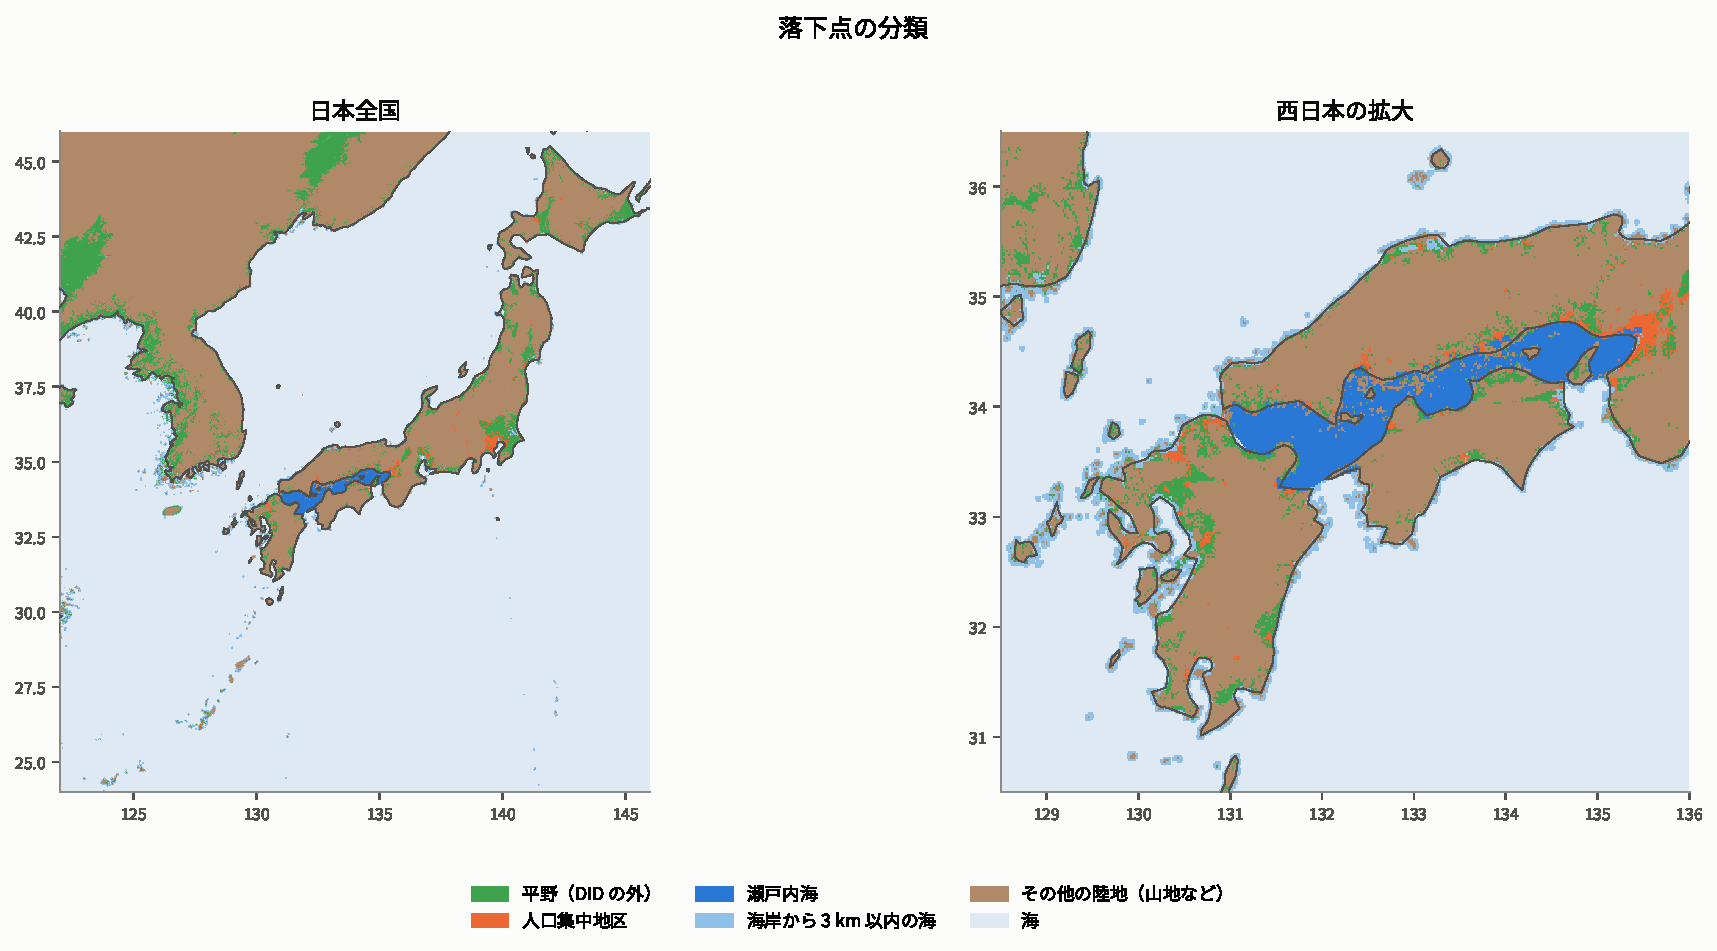
\includegraphics[width=\linewidth]{target_mask.pdf}
\caption{落下の目標。緑が平野（DID の外）、濃い青が瀬戸内海、薄い青が海岸から
\SI{3}{\kilo\metre} 以内の海。赤の人口集中地区と茶の山地は目標に含めない。
右は西日本の拡大。}
\label{fig:target}
\end{figure}

\begin{figure}[htbp]
\centering
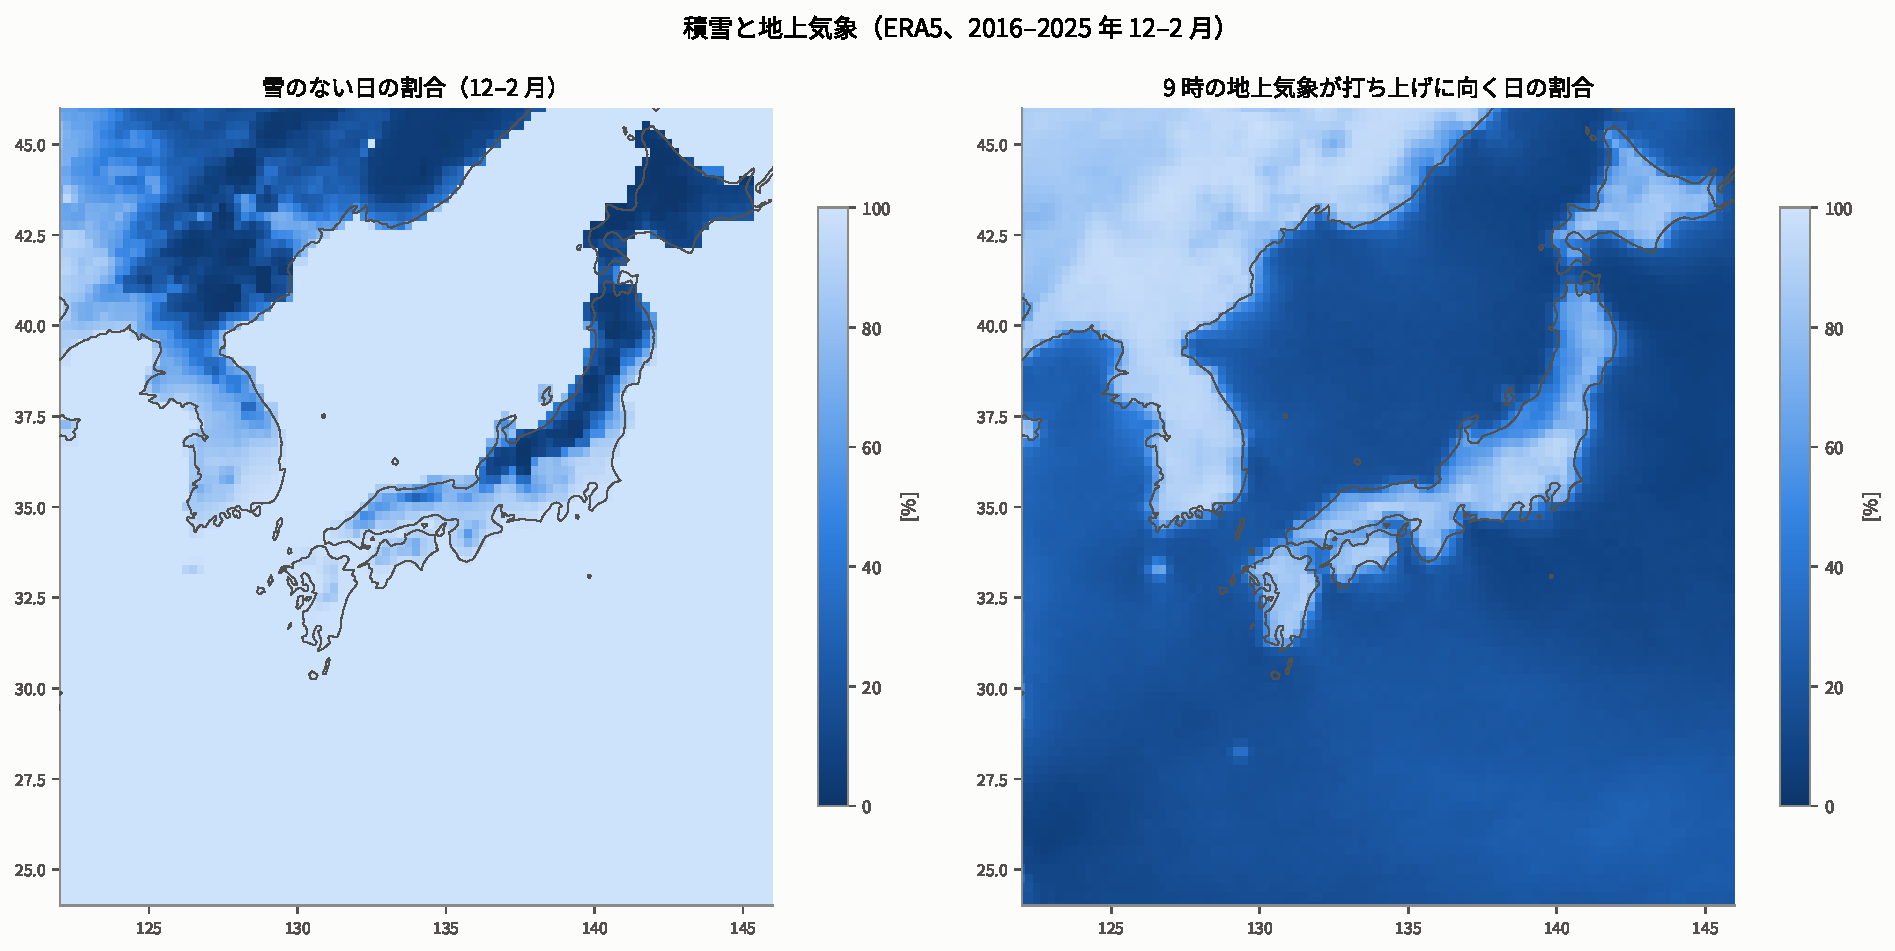
\includegraphics[width=\linewidth]{snow_weather.pdf}
\caption{左: 12--2 月に雪のない日の割合（ERA5、12 時）。右: 9 時の地上気象
（風 \SI{5}{\metre\per\second} 以下・降水 \SI{0.5}{\milli\metre} 未満）が打ち上げに向く日の割合。
日本海側と北日本は雪で、沿岸と島は風で割合が下がる。}
\label{fig:snow}
\end{figure}

\section{日本全国の結果}
\label{sec:japan}

\subsection{冬の気球はどこへ流されるか}

冬の日本の上空には強い西風（ジェット気流）が吹いている。標準の飛行では、
どこから上げても平均で東へ約 \SI{255}{\kilo\metre} 流される（図~\ref{fig:drift}）。
南へ行くほどジェットの芯に近く、流される距離が長い。

このため、打ち上げ地点の\textbf{東 \SIrange{150}{350}{\kilo\metre}} に目標が広がっているかどうかで
結果がほぼ決まる。九州北西部から上げると、その先に瀬戸内海が東西 \SI{400}{\kilo\metre} にわたって
横たわっている。瀬戸内海は冬でも雪がなく、落下点がそこに入れば成功に数える。
これが西日本の北西部が有利になる理由である。

\begin{figure}[htbp]
\centering
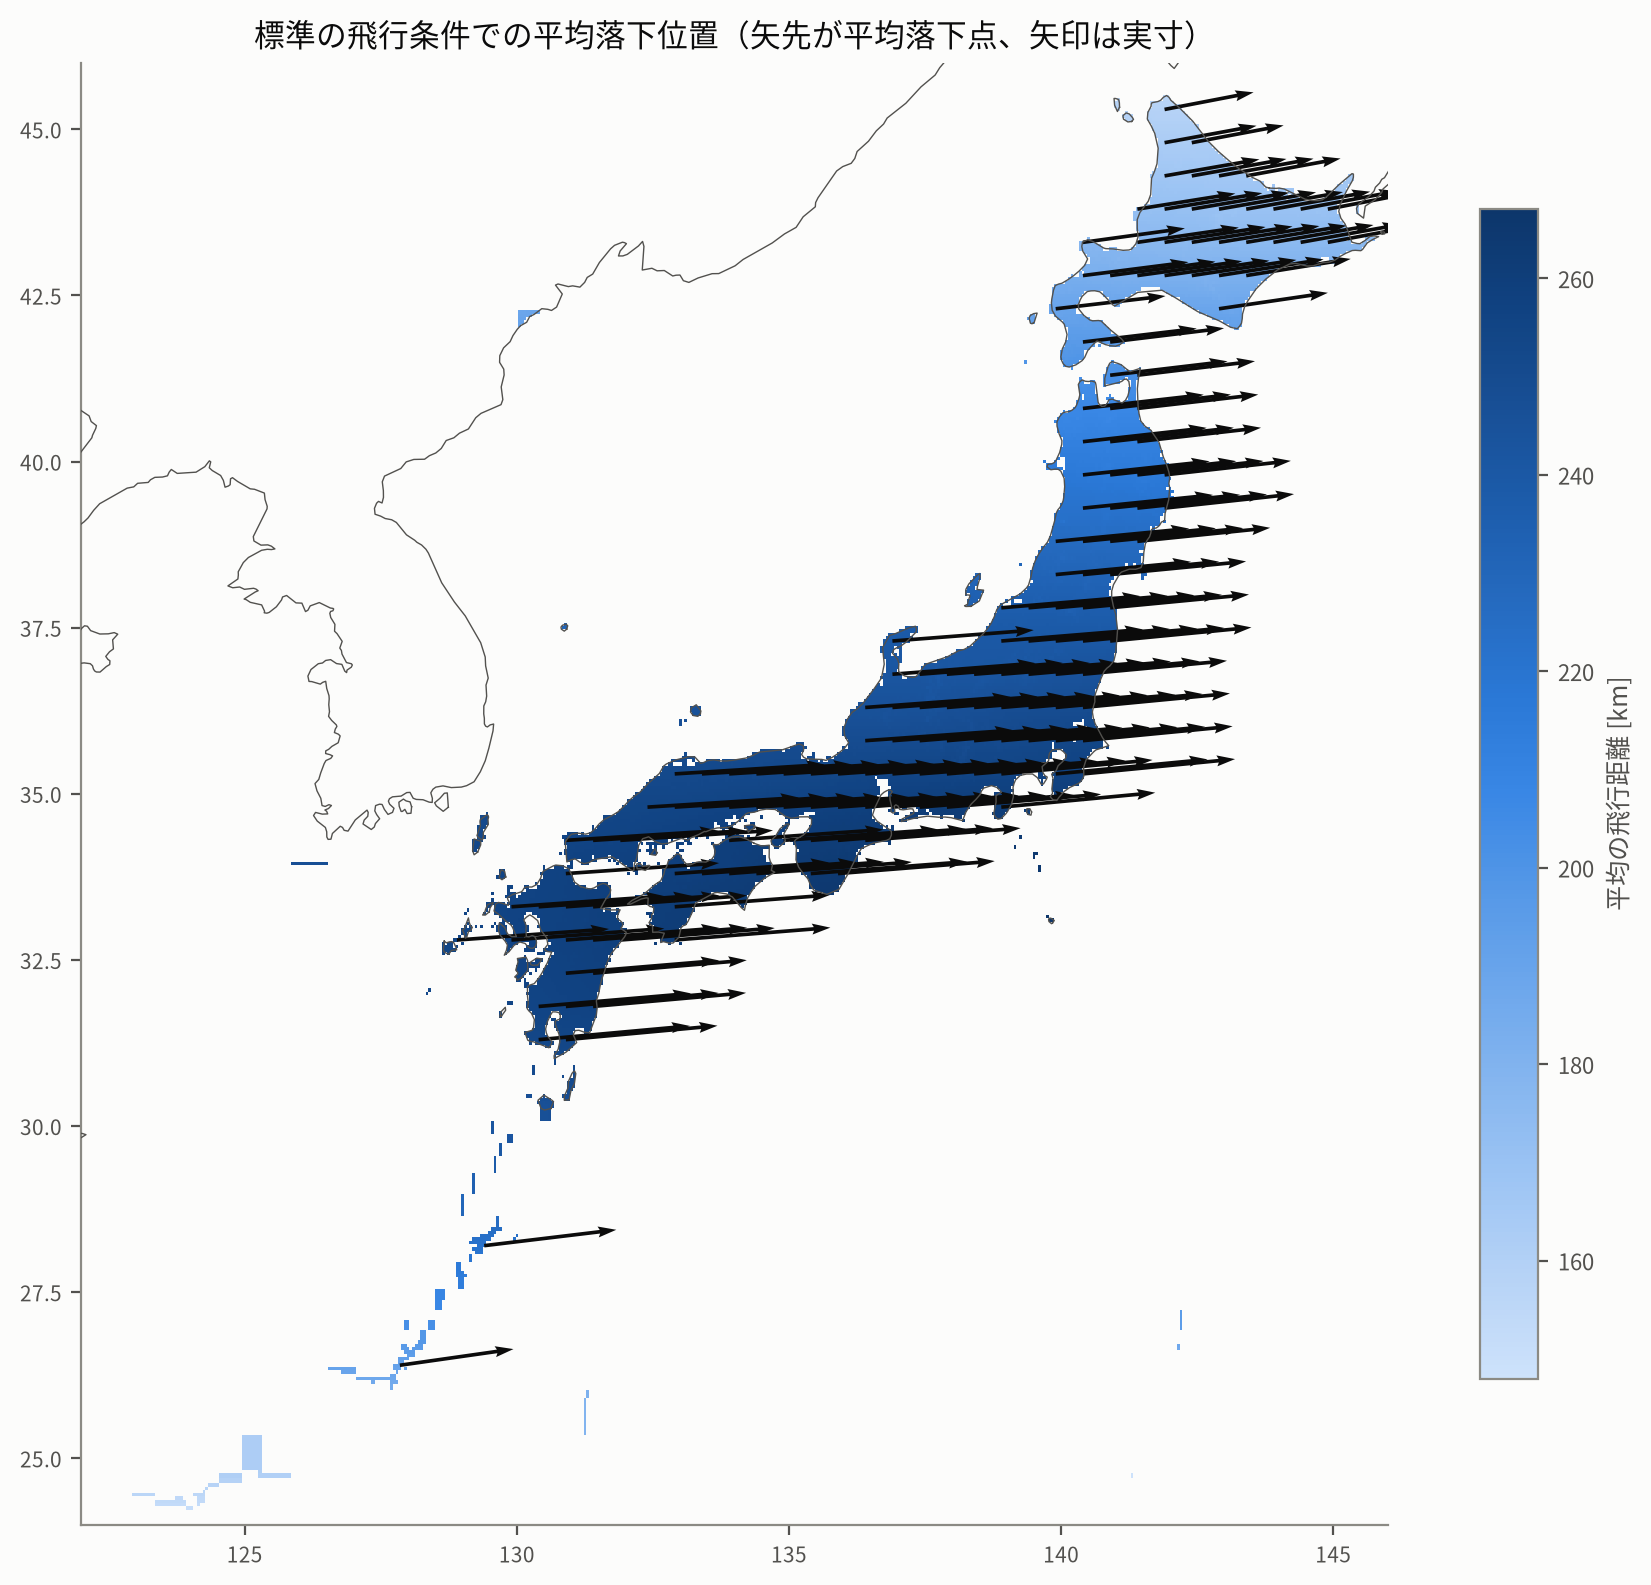
\includegraphics[width=\linewidth]{drift_arrows.png}
\caption{標準の飛行での平均落下位置（903 日の平均）。矢印は実寸で、根元が打ち上げ地点、
矢先が平均の落下点。色は平均の飛行距離。}
\label{fig:drift}
\end{figure}

\subsection{実施できる確率の地図}

図~\ref{fig:pmaps} は、全候補について 4 つの確率を地図にしたものである。
「落下予測が目標に入る」確率（左上）は、九州北西部と山口県で \SIrange{40}{50}{\percent} ある。
ここに雪（右上）と地上気象（左下）の条件を重ねると、実施できる確率（右下）は
最も高い場所でも \SI{33}{\percent} になる。

\begin{figure}[htbp]
\centering
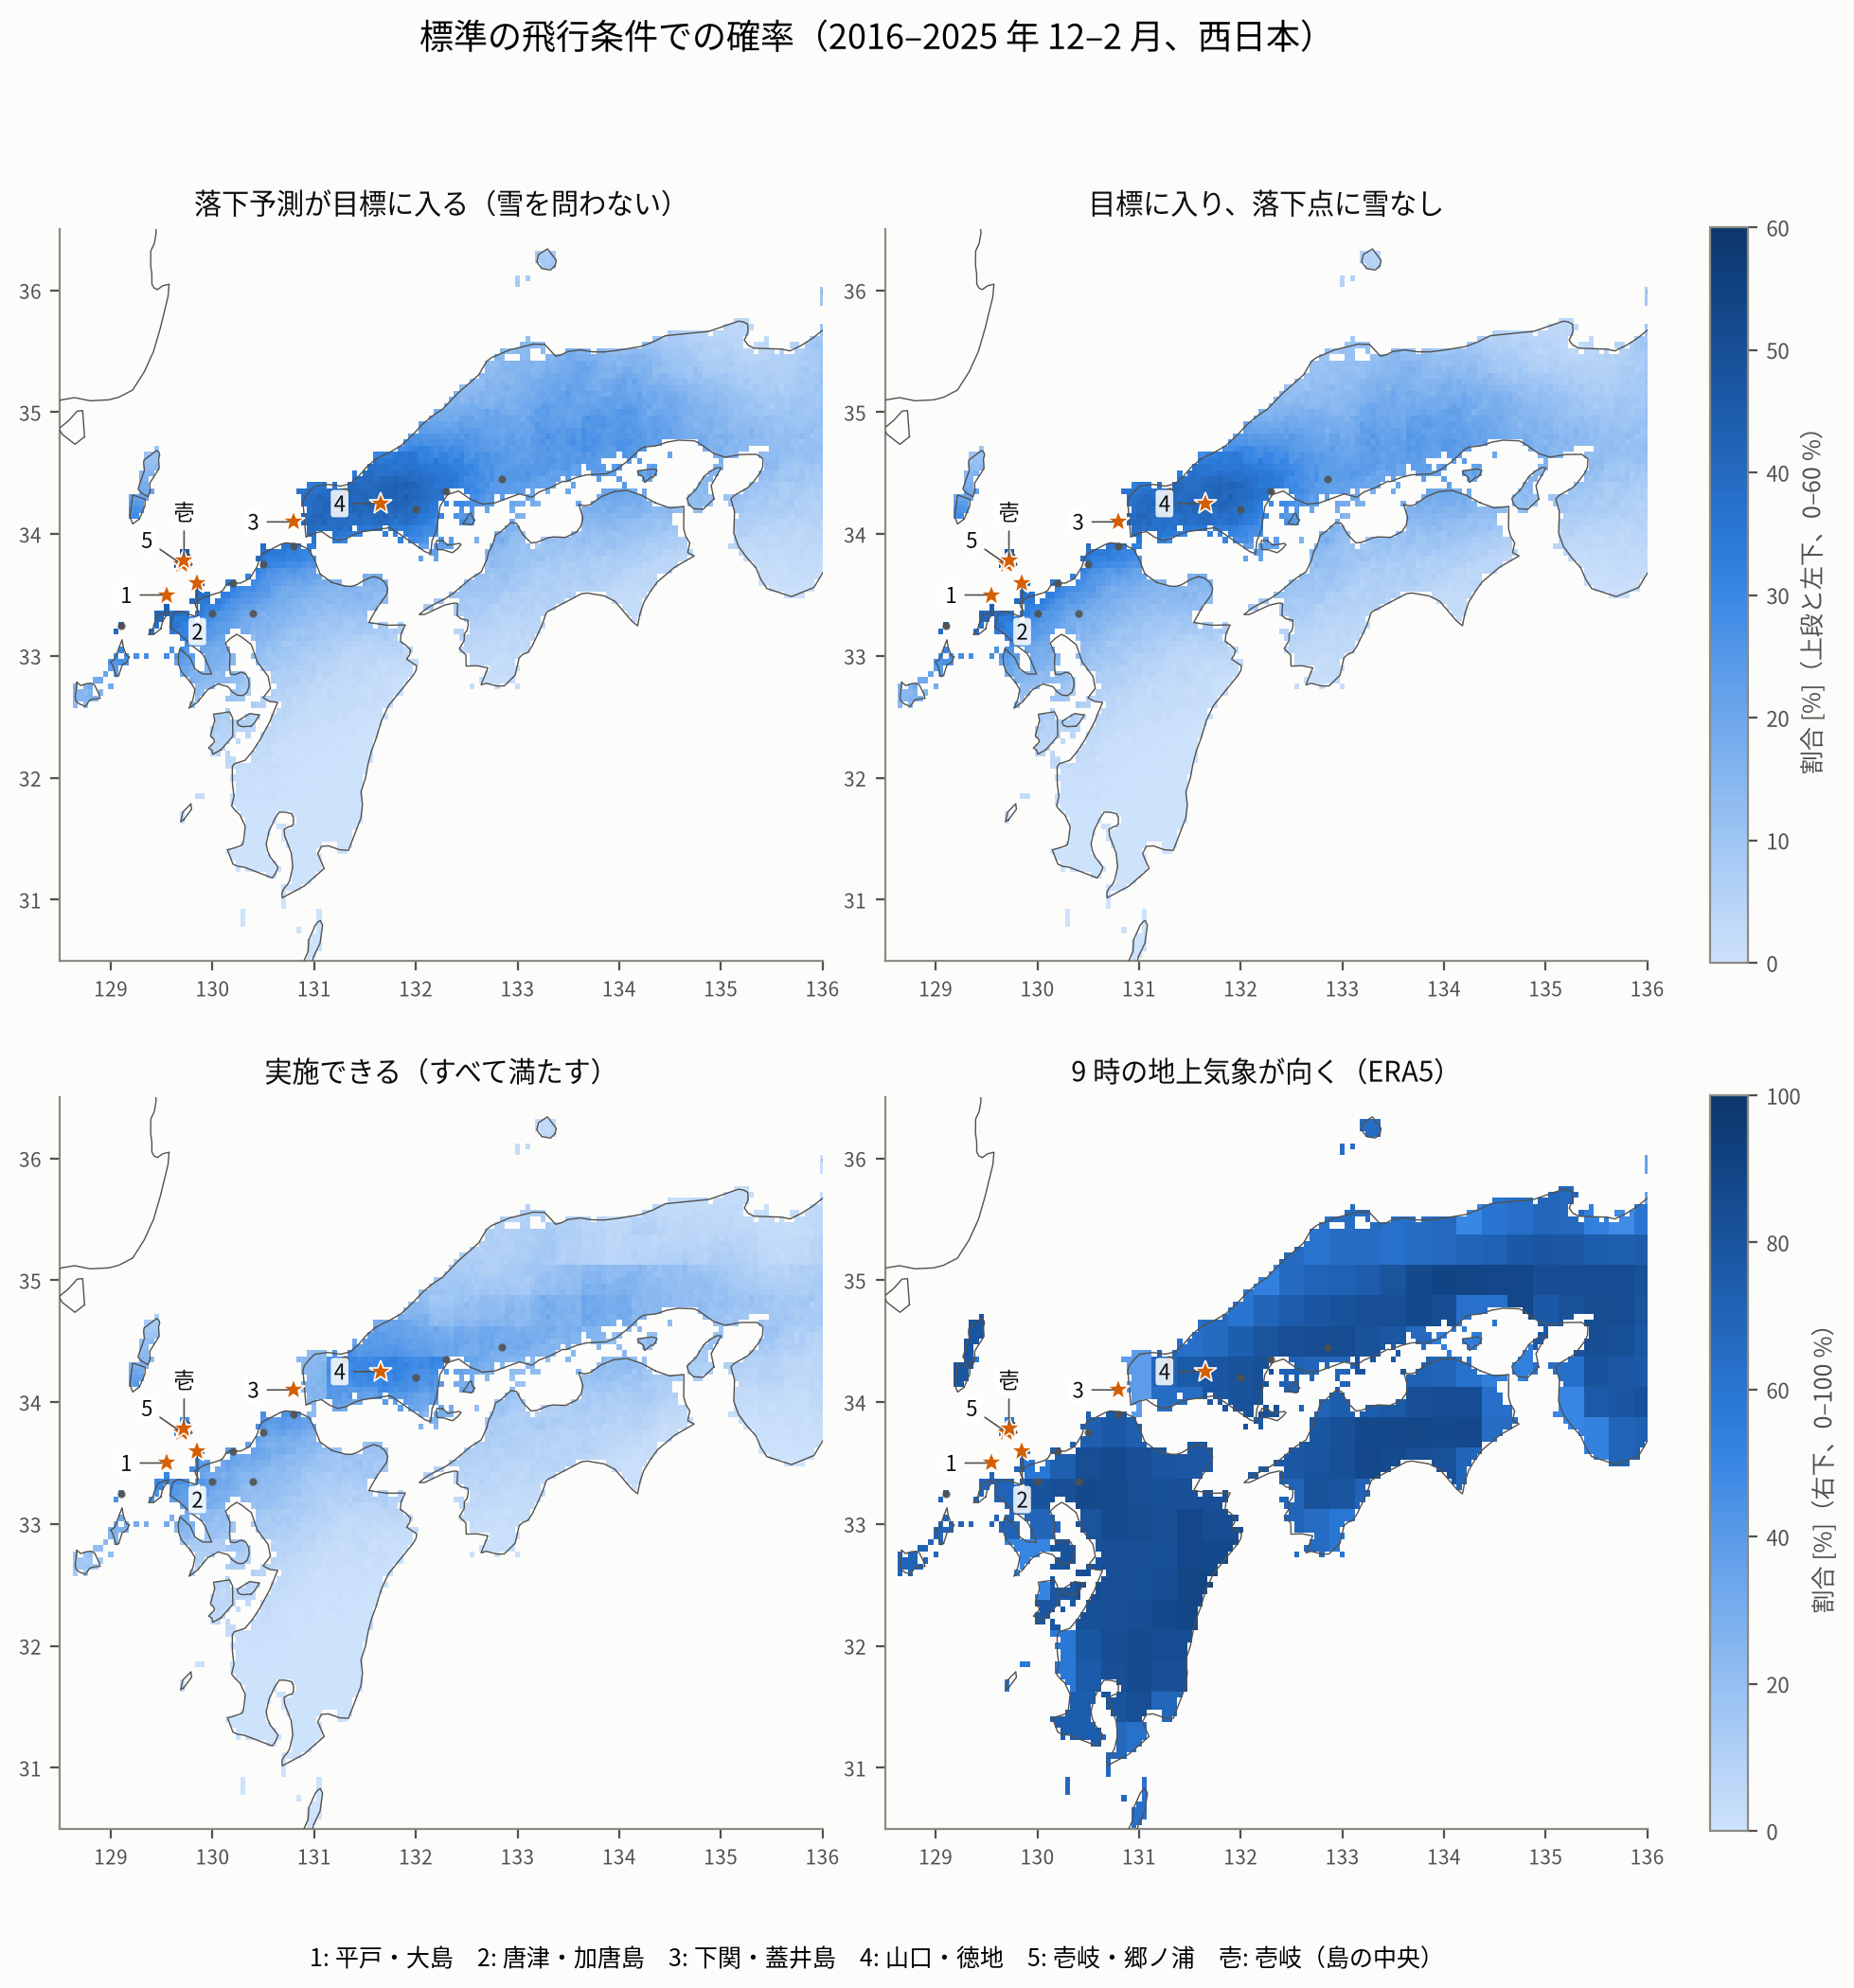
\includegraphics[width=\linewidth]{p_maps_std.png}
\caption{標準の飛行での確率。左上: 落下予測が目標に入る（雪を問わない）。
右上: 加えて落下点に雪がない。左下: 9 時の地上気象が向く。右下: すべてを満たす（実施できる）。
番号は上位の候補地。}
\label{fig:pmaps}
\end{figure}

地方ごとに最も高い地点を表~\ref{tab:region} にまとめた。北海道・東北は打ち上げ地点の雪で、
関東は落下点が太平洋の沖に出るため、ほとんど実施できない。
短時間の飛行にすると、飛行距離が縮んで中国地方や四国の瀬戸内海側でも瀬戸内海・
平野に落ちるようになり、各地の確率が上がる（図~\ref{fig:pshort}）。

\begin{table}[htbp]
\centering
\small
\caption{地方ごとの最も高い地点（打ち上げ地点の標高 \SI{200}{\metre} 以下、飛行条件のばらつきなし）。}
\label{tab:region}
\begin{tabular}{lcrcr}
\toprule
& \multicolumn{2}{c}{標準の飛行} & \multicolumn{2}{c}{短時間の飛行} \\
地方 & 地点 & 実施 [\%] & 地点 & 実施 [\%] \\
\midrule
北海道 & 42.80, 143.20 & 3 & 43.15, 143.65 & 5 \\
東北 & 37.80, 139.10 & 2 & 37.95, 139.10 & 4 \\
関東 & 36.25, 138.90 & 5 & 36.25, 138.90 & 20 \\
中部・東海 & 35.50, 137.05 & 27 & 35.30, 138.45 & 25 \\
近畿 & 34.85, 134.50 & 15 & 34.75, 134.85 & 27 \\
四国 & 34.00, 132.15 & 23 & 34.40, 133.00 & 37 \\
中国 & 34.35, 131.30（長門） & 32 & 34.45, 132.85（東広島） & 44 \\
九州・壱岐・対馬 & 33.50, 129.55（平戸・大島） & \textbf{33} & 33.60, 130.20（糸島） & \textbf{51} \\
南西諸島 & 24.45, 122.95 & 5 & 26.35, 126.80 & 13 \\
\bottomrule
\end{tabular}
\end{table}

\begin{figure}[htbp]
\centering
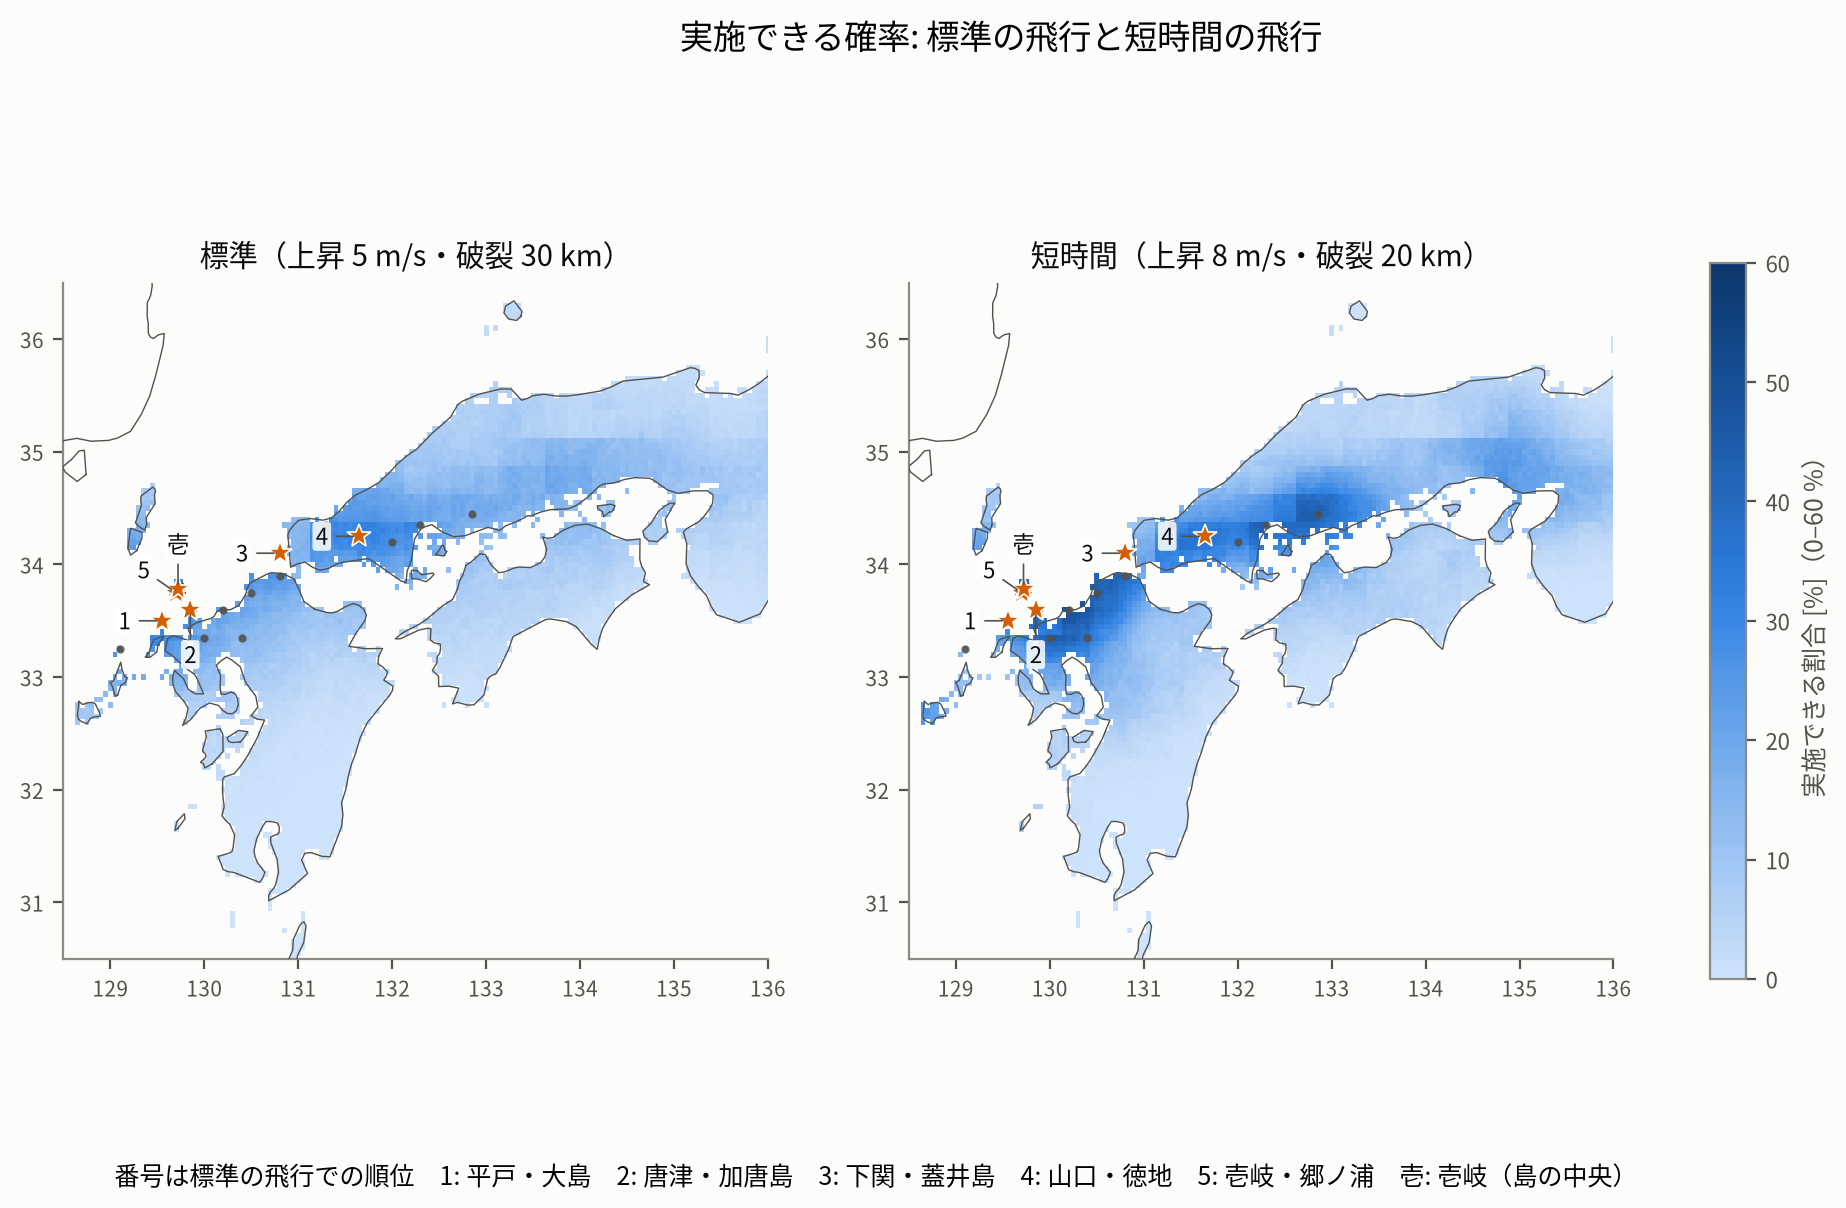
\includegraphics[width=\linewidth]{p_maps_short.png}
\caption{実施できる確率の比較。左が標準の飛行、右が短時間の飛行。}
\label{fig:pshort}
\end{figure}

\begin{figure}[htbp]
\centering
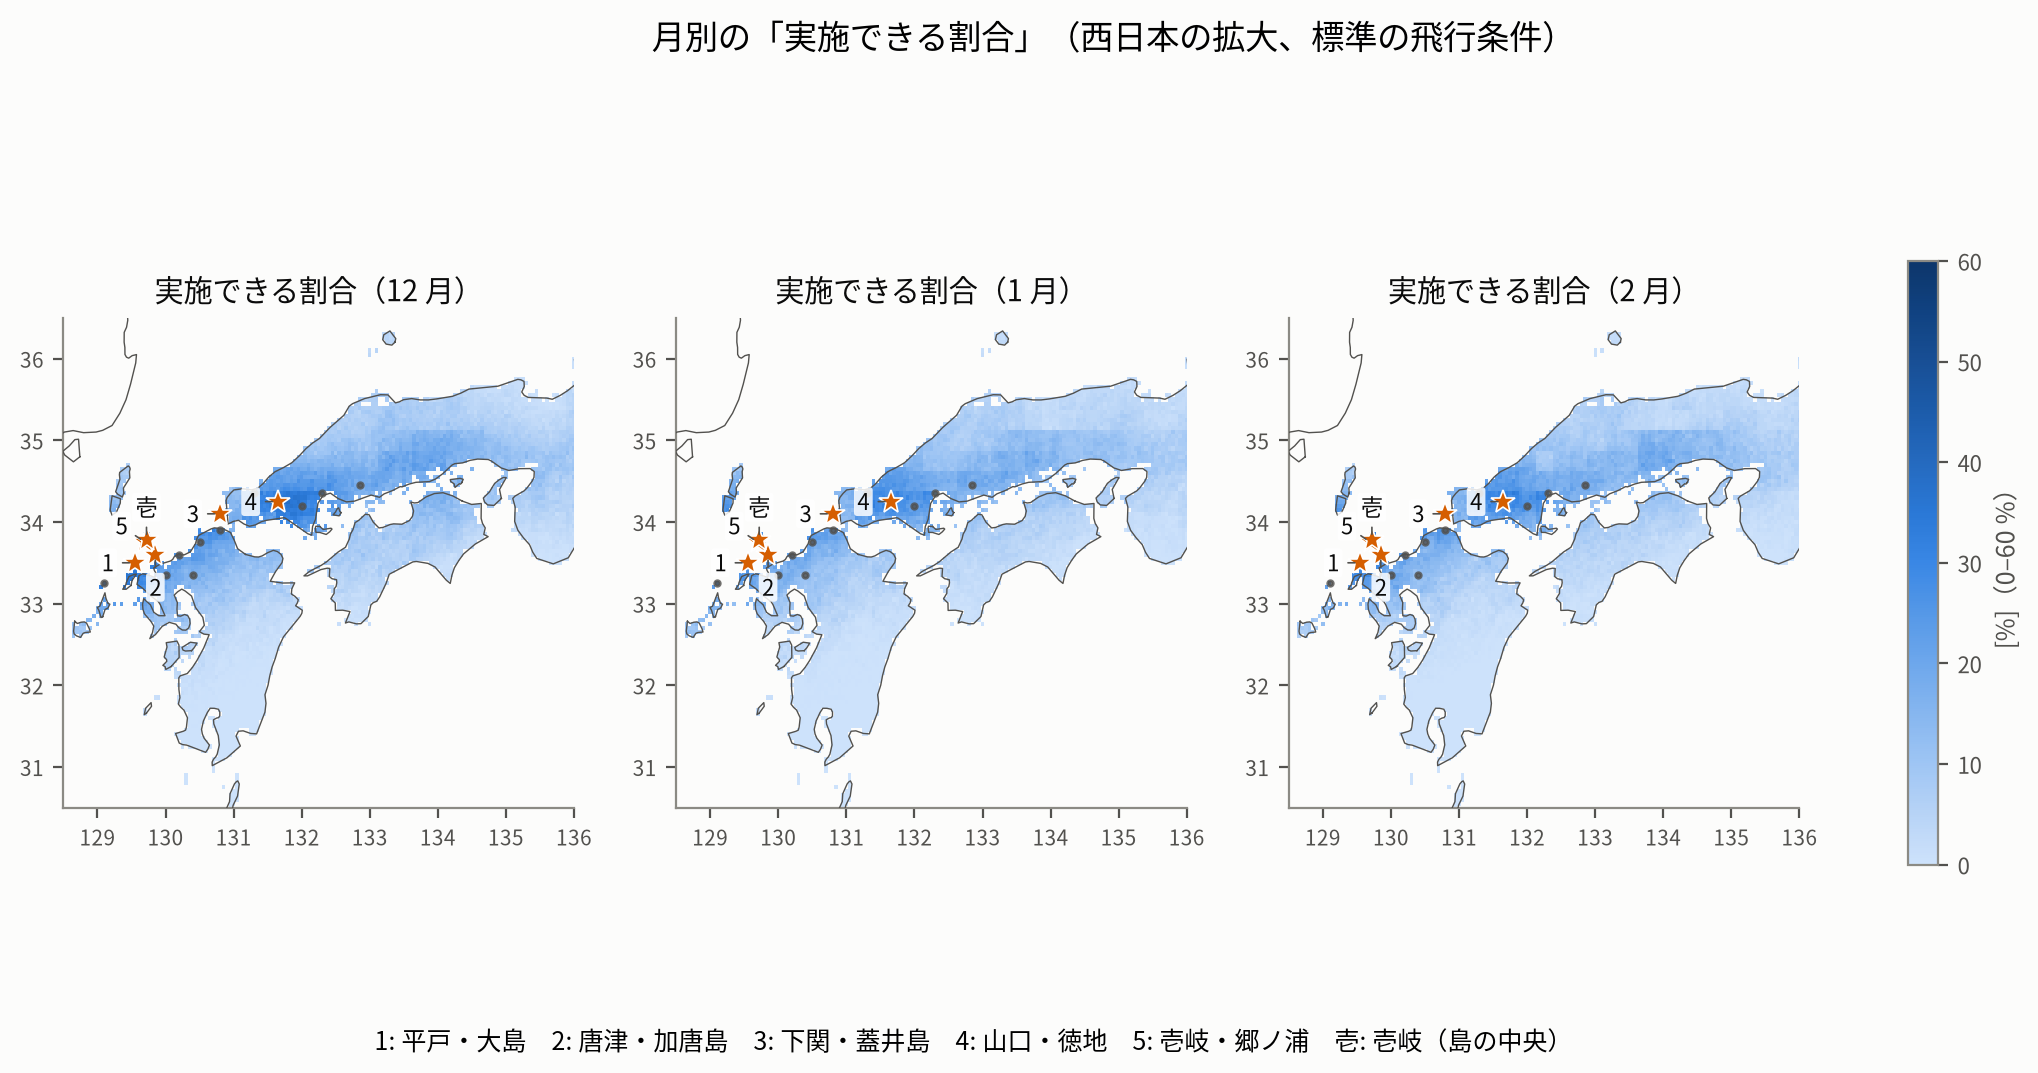
\includegraphics[width=\linewidth]{p_total_months.png}
\caption{標準の飛行で実施できる確率の月ごとの違い。}
\label{fig:months}
\end{figure}

\section{上位の候補地}
\label{sec:sites}

\subsection{候補地の比べ方}

全候補の地図から、互いに \SI{30}{\kilo\metre} 以上離れた上位の地点を、標準と短時間の
飛行のそれぞれで 8 地点ずつ選び、壱岐の 2 地点を加えた 16 地点で、飛行条件の
ばらつき（64 通り）を入れて計算し直した。地点名は最寄りの地名である。

\begin{table}[htbp]
\centering
\scriptsize
\caption{候補地ごとの確率。「落下」は落下予測が目標に入る確率（雪を問わない、標準の飛行）、
「雪なし」は打ち上げ地点に雪がない確率、「地上気象」は 9 時の風・雨が向く確率。
右の 2 列が 4 条件をすべて満たす「実施できる」確率で、括弧内は年ごとのブロック・
ブートストラップによる 95\% 区間。標準の飛行の順に並べた。}
\label{tab:sites}
\resizebox{\linewidth}{!}{\begin{tabular}{lcrrrcc}
\toprule
候補地 & 緯度, 経度 & 落下 & 雪なし & 地上気象 & \multicolumn{2}{c}{実施できる確率 [\%]} \\
& & [\%] & [\%] & [\%] & 標準 (95\% 区間) & 短時間 (95\% 区間) \\
\midrule
平戸・大島 & 33.50, 129.55 & 47 & 99 & 70 & \textbf{33} (30--35) & \textbf{34} (30--37) \\
唐津・加唐島 & 33.60, 129.85 & 44 & 99 & 70 & \textbf{32} (29--35) & \textbf{45} (42--48) \\
下関・蓋井島 & 34.10, 130.80 & 40 & 98 & 77 & \textbf{31} (29--33) & \textbf{36} (34--38) \\
山口・徳地 & 34.25, 131.65 & 41 & 90 & 79 & \textbf{30} (28--33) & \textbf{35} (33--38) \\
壱岐・郷ノ浦 & 33.75, 129.70 & 49 & 98 & 59 & \textbf{30} (27--32) & \textbf{38} (35--42) \\
壱岐（島の中央） & 33.78, 129.72 & 48 & 98 & 59 & \textbf{29} (26--32) & \textbf{38} (35--42) \\
廿日市 & 34.35, 132.30 & 36 & 93 & 83 & \textbf{28} (27--30) & \textbf{43} (40--45) \\
長門・三隅 & 34.35, 131.30 & 40 & 96 & 70 & \textbf{28} (25--30) & \textbf{26} (24--28) \\
佐世保・宇久島 & 33.25, 129.10 & 40 & 99 & 70 & \textbf{27} (25--29) & \textbf{15} (13--17) \\
岩国 & 34.20, 132.00 & 38 & 81 & 81 & \textbf{27} (24--29) & \textbf{31} (28--34) \\
北九州・若松 & 33.90, 130.80 & 35 & 98 & 77 & \textbf{26} (24--28) & \textbf{39} (37--42) \\
糸島・志摩 & 33.60, 130.20 & 35 & 94 & 73 & \textbf{24} (21--28) & \textbf{48} (45--51) \\
唐津・相知 & 33.35, 130.00 & 30 & 99 & 81 & \textbf{23} (20--27) & \textbf{42} (40--45) \\
福津 & 33.75, 130.50 & 33 & 96 & 73 & \textbf{23} (20--26) & \textbf{44} (40--46) \\
東広島 & 34.45, 132.85 & 26 & 87 & 85 & \textbf{20} (18--22) & \textbf{42} (38--45) \\
吉野ヶ里 & 33.35, 130.40 & 20 & 99 & 87 & \textbf{16} (13--19) & \textbf{37} (35--40) \\
\bottomrule
\end{tabular}
}
\end{table}

\begin{figure}[htbp]
\centering
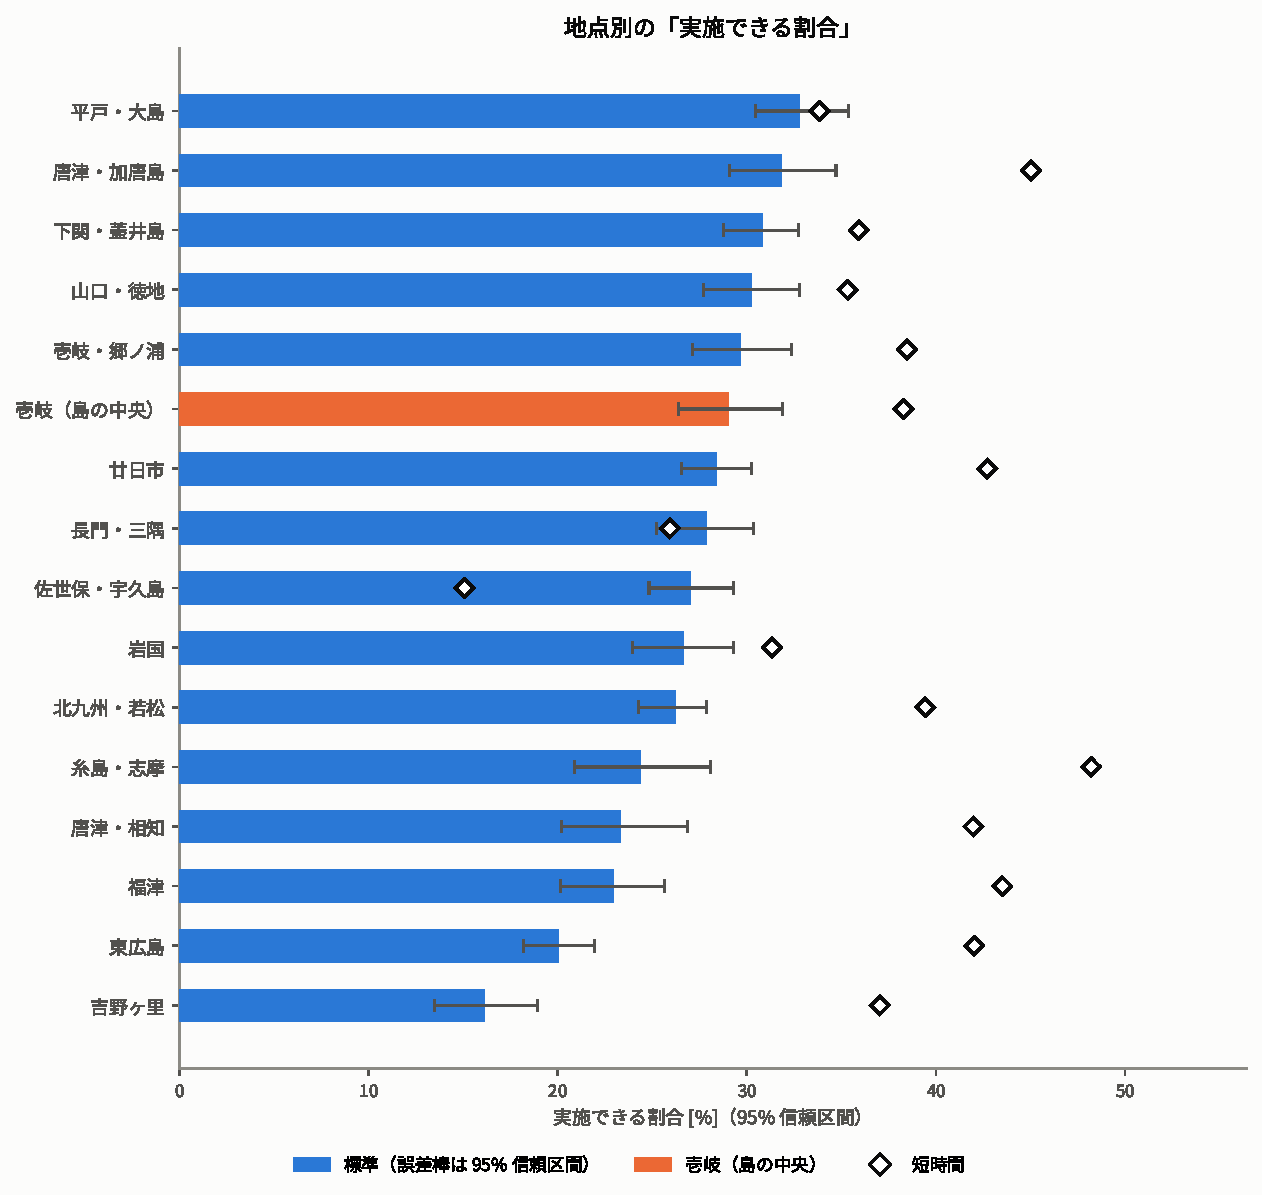
\includegraphics[width=\linewidth]{ranking.pdf}
\caption{実施できる確率の順位（95\% 区間つき）。丸が標準の飛行、四角が短時間の飛行。}
\label{fig:ranking}
\end{figure}

標準の飛行では、平戸・大島（\SI{33}{\percent}）、唐津・加唐島（\SI{32}{\percent}）、
下関・蓋井島（\SI{31}{\percent}）、山口・徳地（\SI{30}{\percent}）、壱岐（\SI{29}{\percent}）が
上位に並ぶ。95\% 区間はおよそ $\pm$\SI{3}{\percent} で、上位 5 地点の差は区間の中に収まる。
つまり標準の飛行では、\textbf{九州北西部から山口県のどこでも、ほぼ同じ 3 割}と考えてよい。
地上気象をアメダスで判定し直すと、壱岐・唐津・平戸はそれぞれ \SIrange{2}{8}{\percent} 上がる（\ref{sec:amedas} 節）。

短時間の飛行では差がはっきりする。糸島・志摩（\SI{48}{\percent}）と唐津・加唐島（\SI{45}{\percent}）が
抜け出し、壱岐（\SI{38}{\percent}）との差は区間の外にある。飛行距離が \SI{180}{\kilo\metre} に縮むと、
糸島や唐津から上げた気球は瀬戸内海の西半分（周防灘・伊予灘）にちょうど落ちる。
ただし落下予測だけを比べると、壱岐（\SI{62}{\percent}）と糸島（\SI{65}{\percent}）の差は小さい。
差の大部分は 9 時の地上気象で、壱岐は \SI{59}{\percent}、糸島は \SI{71}{\percent} の日しか向かない。
地上気象の評価は \ang{0.25} 格子の ERA5 によるもので、島では不確かさが大きい（\ref{sec:amedas} 節）。

\subsection{落下点の散らばり}

図~\ref{fig:clouds} は、上位の地点と壱岐の落下点を 903 日 $\times$ 64 本すべて描いたものである。
落下点は東西に長い帯になり、その帯の半分ほどが瀬戸内海に重なる。成功の大部分は
瀬戸内海への着水で、平野への着地は数 \% にすぎない（図~\ref{fig:breakdown}）。
\textbf{瀬戸内海への着水を認めるかどうかで、結論はほぼ決まる}。認めない場合は
\ref{sec:sensitivity} 節の感度を参照のこと。

\begin{figure}[htbp]
\centering
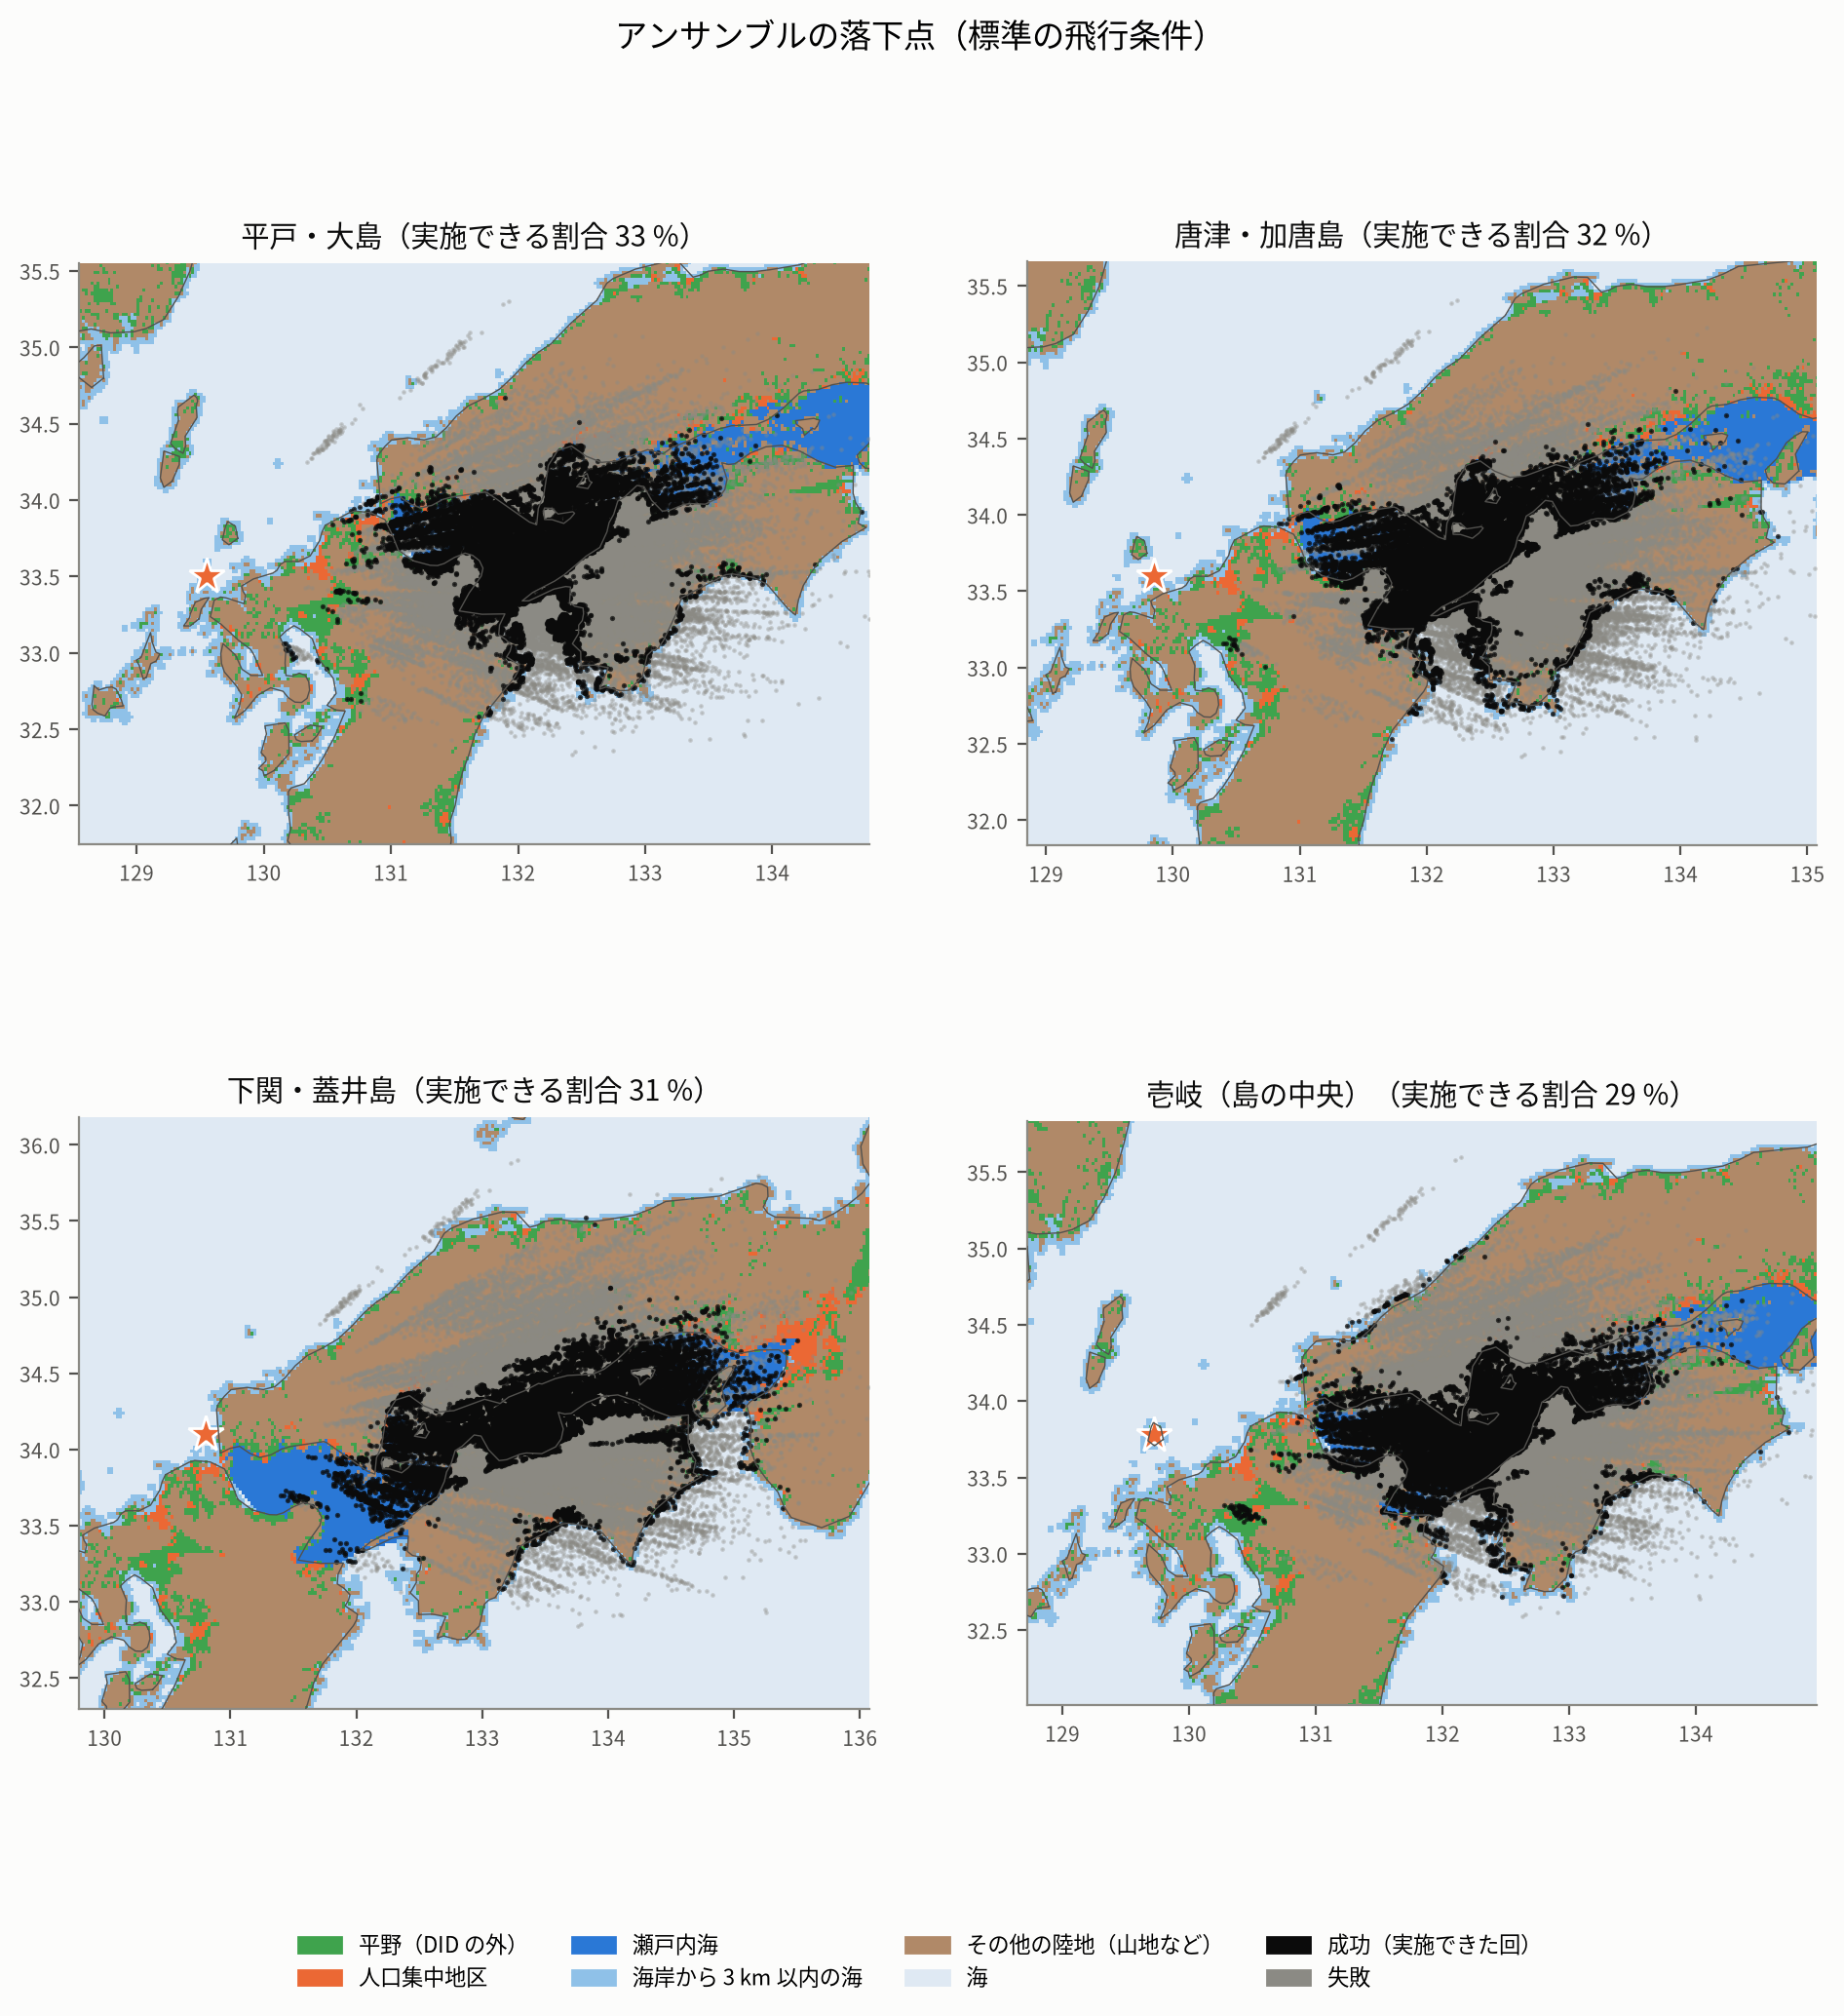
\includegraphics[width=\linewidth]{landing_clouds.png}
\caption{落下点の散らばり（標準の飛行、903 日 $\times$ 64 本）。黒が実施できた回、灰が
それ以外（雪・地上気象で中止の日も含む）。星が打ち上げ地点。各図の題の割合は地上気象を ERA5 で判定した値（壱岐のアメダスでの値は \ref{sec:amedas} 節）。}
\label{fig:clouds}
\end{figure}

\begin{figure}[htbp]
\centering
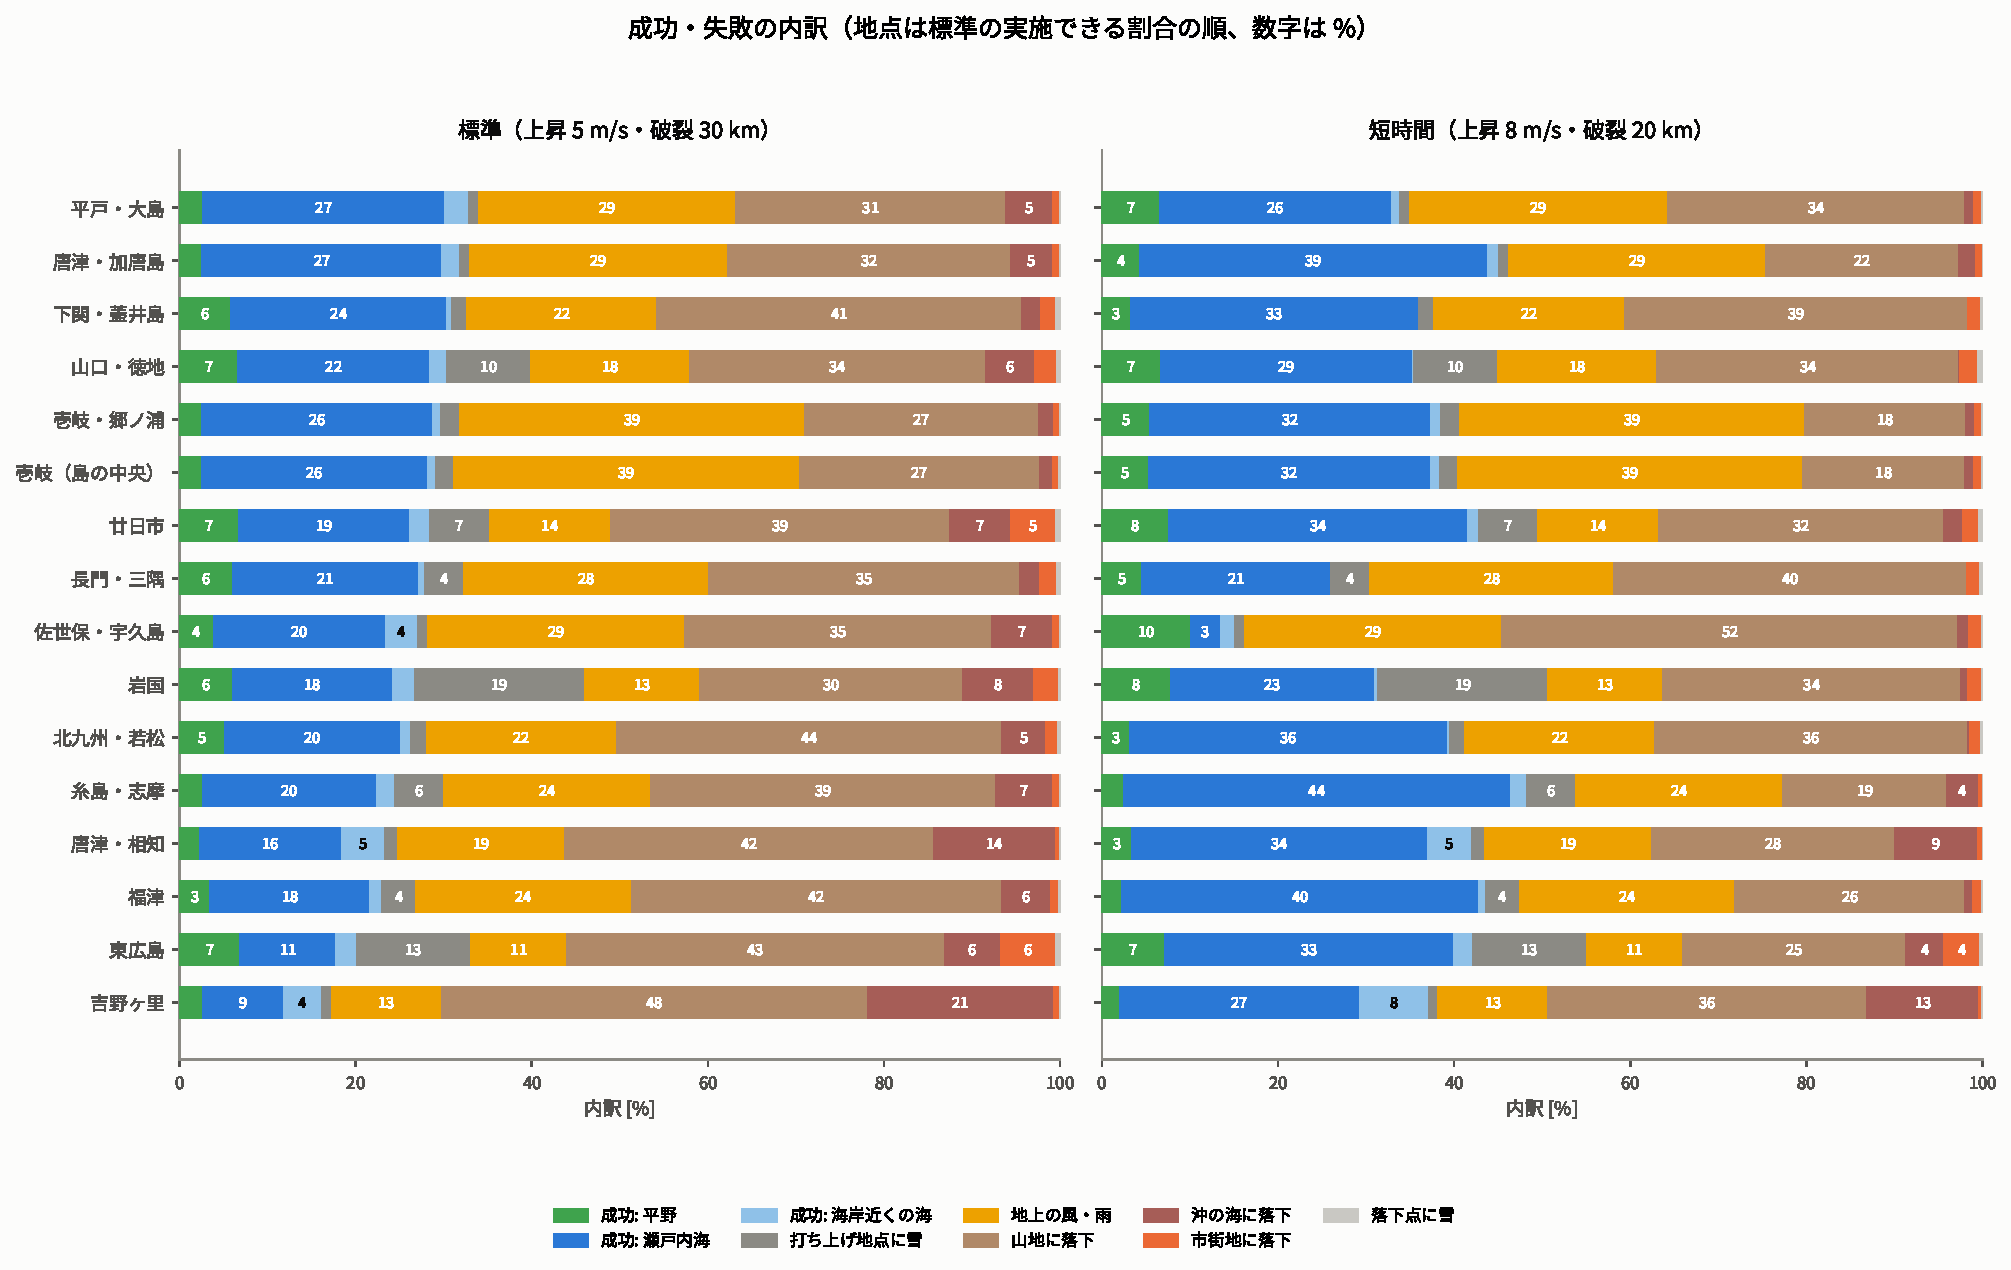
\includegraphics[width=\linewidth]{breakdown.pdf}
\caption{9 時の判断の結果の内訳。左から成功（瀬戸内海・平野・海岸近くの海）、
右へ中止・見送りの理由。雪 → 地上気象 → 落下予測の順に判断したときの割合で、
合計は \SI{100}{\percent}。}
\label{fig:breakdown}
\end{figure}

\subsection{島と本土}

上位には加唐島・蓋井島・平戸の大島・宇久島のような小さな島が入っている。
島は冬でも雪がほとんどなく、地上気象の格子の選び方によっては値が高く出やすい。

実際に機材を運ぶ手間を考えると、近くの本土も比べておく必要がある（格子の値、飛行条件の
ばらつきなし）。
\begin{itemize}
  \item 加唐島の対岸の\textbf{呼子（唐津市、33.55, 129.85）}は標準 \SI{30}{\percent}・
    短時間 \SI{44}{\percent} で、加唐島（32・45）とほとんど変わらない。
  \item 平戸・大島の代わりに\textbf{平戸島}（33.35--33.40, 129.50--129.55）を使うと、
    標準 \SI{30}{\percent}、短時間 \SIrange{23}{29}{\percent} である。
  \item 蓋井島の対岸（下関市吉見付近）は \SIrange{15}{16}{\percent} まで下がる。
    落下予測（\SI{39}{\percent}）は蓋井島（\SI{41}{\percent}）とほぼ同じで、差は地上気象
    （対岸 \SI{39}{\percent}、蓋井島 \SI{77}{\percent}）から来ている。これは両者で参照した ERA5 の
    格子が違うためで、実際の風の差をどこまで表しているかは分からない。
  \item 宗像・福津（33.75--33.85, 130.50--130.60）は標準 \SIrange{20}{26}{\percent}、
    短時間 \SIrange{40}{45}{\percent} で、短時間の飛行なら上位と同等になる。
\end{itemize}

\subsection{打ち上げに使えそうな広場}
\label{sec:osm}

格子の計算で分かるのは「どのあたりから上げるとよいか」までで、実際にどの広場で
上げるかは別に探す必要がある。そこで OpenStreetMap から、壱岐島の全域と、上位の候補地の
半径 \SI{12}{\kilo\metre} 以内（呼子・平戸島・下関の本土側などを含む）にある
公園・グラウンド・競技場・学校の校庭・草地を集めた。

広場ごとに、敷地の中で電線・電柱・建物・鉄塔・林から最も離れられる点を探し、
その距離（ここでは「距離」と呼ぶ）を求めた。面積 \SI{0.3}{\hectare} 以上で、この距離が
\SI{40}{\metre} 以上の所を候補とし、空港の滑走路から \SI{3}{\kilo\metre} 以内は除いた。
同じ学校の敷地とグラウンドのように重なるものは 1 つにまとめた。
さらに、その点から上げたときの実施できる確率を、\ref{sec:method} 節と同じ方法（飛行条件 64 通り、
地上気象は近くにアメダスがあればアメダス）で広場ごとに計算した。

候補は 9 地域で 674 か所あった（表~\ref{tab:spotgroups}、図~\ref{fig:spotswest}）。
同じ地域の中では、確率は広場によってあまり変わらない。たとえば壱岐の 34 か所は、
標準の飛行でどれも \SIrange{36}{38}{\percent} である。場所の良し悪しは地域でほぼ決まり、
地域の中では、電線や建物から離れられるか、使う許可が取れるかで選べばよい。

\begin{table}[htbp]
\centering
\small
\caption{地域ごとの打ち上げ候補地（OpenStreetMap、2026 年 9 月時点）。「距離」は電線・建物・林までの距離。
確率の幅はその地域の候補地の最小〜最大。地上気象は壱岐・平戸・唐津はアメダス、その他は ERA5
（ERA5 は沿岸で確率が低めに出る）。一覧は \texttt{results/launch\_spots.csv}（Google マップのリンクつき）。}
\label{tab:spotgroups}
\resizebox{\linewidth}{!}{\begin{tabular}{lrrccl}
\toprule
地域 & 候補 & 距離 60 m 以上 & 標準 [\%] & 短時間 [\%] & 距離がいちばん大きい所 \\
\midrule
壱岐 & 34 & 10 & 36--38 & 45--50 & 壱岐市立芦辺中学校（110 m） \\
唐津・呼子 & 33 & 20 & 28--35 & 46--51 & （付近: 相賀）（178 m） \\
平戸 & 10 & 6 & 27--34 & 27--35 & 千里ヶ浜鄭成功記念公園（152 m） \\
長門 & 26 & 23 & 23--30 & 20--30 & （付近: 阿武川）（330 m） \\
北九州 & 231 & 188 & 14--28 & 20--42 & 西山公園（698 m） \\
唐津・相知 & 81 & 44 & 19--27 & 37--47 & （付近: 国道202号）（142 m） \\
宗像・福津 & 120 & 103 & 19--27 & 39--45 & （付近: 広陵台五丁目）（512 m） \\
糸島 & 113 & 66 & 20--26 & 39--49 & （名前なし）（237 m） \\
下関 & 26 & 23 & 15--16 & 13--18 & （付近: 豊浦養護学校）（303 m） \\
\bottomrule
\end{tabular}
}
\end{table}

\begin{figure}[htbp]
\centering
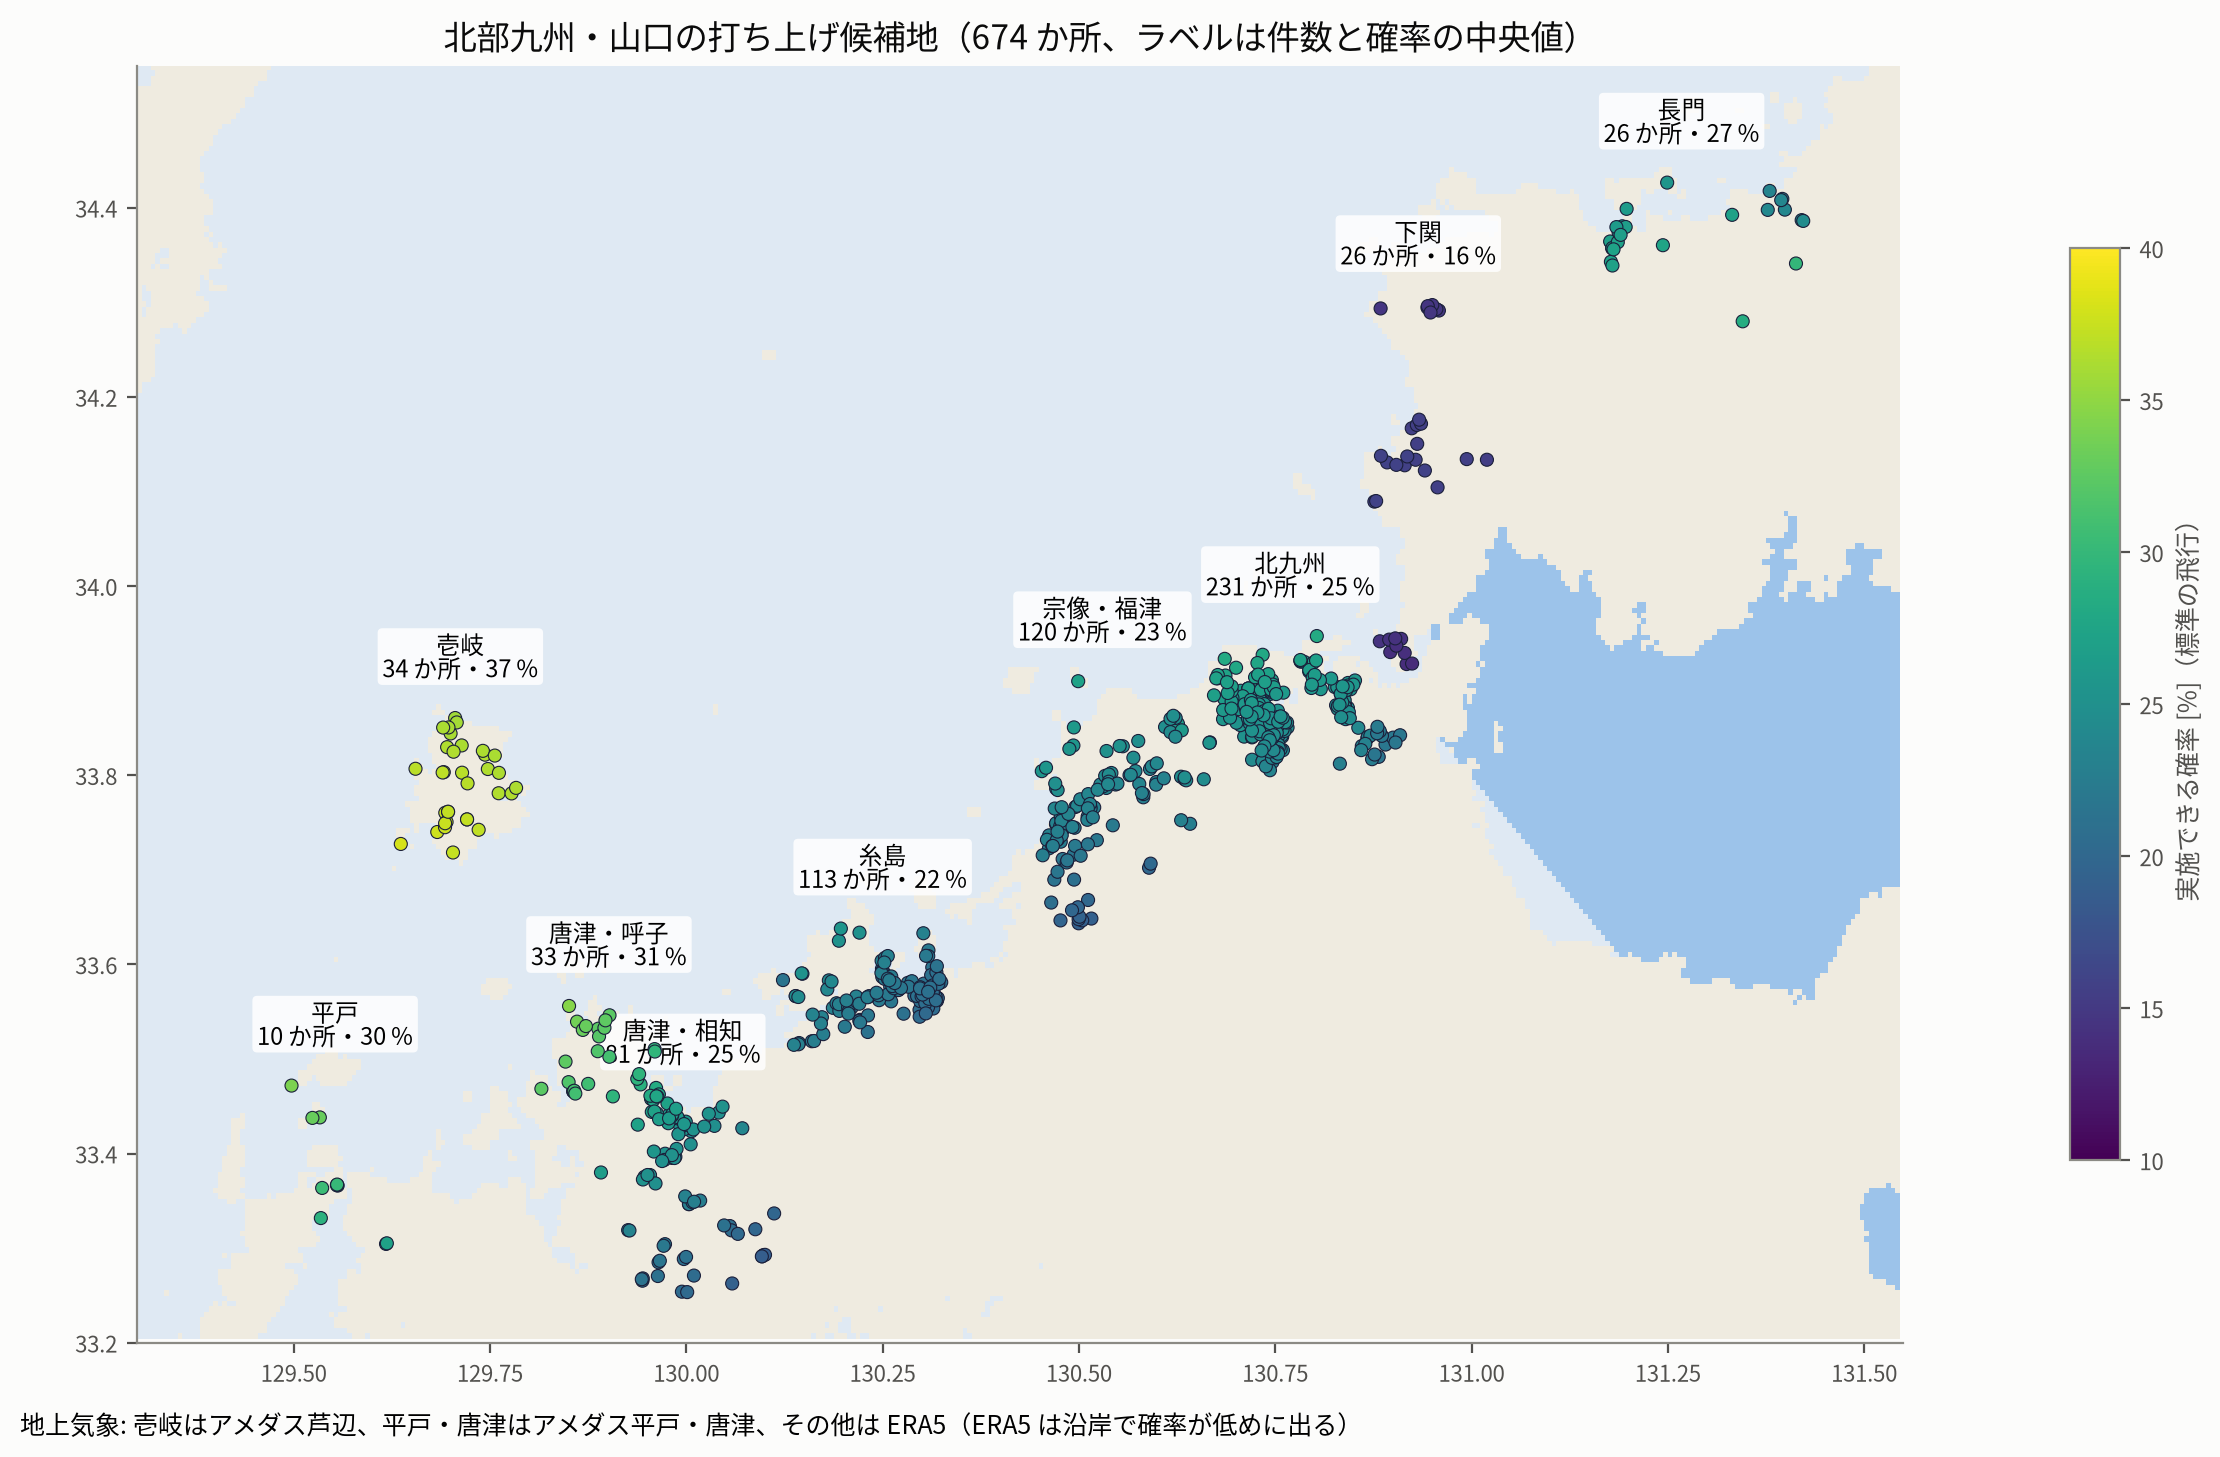
\includegraphics[width=\linewidth]{launch_spots_west.png}
\caption{北部九州・山口の打ち上げ候補地 674 か所。色は標準の飛行で実施できる確率。}
\label{fig:spotswest}
\end{figure}

OpenStreetMap の電線は、地方ではまだ登録が少ない。ここでの「距離」は上限で、実際には
もっと近くに配電線がある可能性が高い。学校の校庭は使用の許可が要る。
一覧は下見の候補を絞るためのもので、使う前に航空写真と現地で電線・建物・立ち入りの可否を
確かめる必要がある。

\section{壱岐から上げた場合}
\label{sec:iki}

\subsection{地上気象の資料で結果が変わる}
\label{sec:amedas}

壱岐は面積約 \SI{130}{\square\kilo\metre} の島で、ERA5 の \ang{0.25} 格子では島のある格子の
\SI{96}{\percent} 以上が海になる。そのまま使うと海上の風になり、9 時に風が
\SI{5}{\metre\per\second} 以下の日は \SI{27}{\percent} しかない（格子の中央値 \SI{6.9}{\metre\per\second}）。
本文の地図と表では、これを避けるために最寄りの「陸が半分以上の格子」を使った。
壱岐の場合、その格子は約 \SI{40}{\kilo\metre} 離れた唐津市の内陸にある。

どちらが実際に近いかを確かめるため、壱岐の芦辺と、平戸・唐津のアメダスの 9 時の観測
（903 日）と比べた（図~\ref{fig:amedas}）。
\begin{itemize}
  \item 芦辺で 9 時の地上気象が打ち上げに向く日は \SI{77}{\percent}（風 \SI{5}{\metre\per\second} 以下が \SI{86}{\percent}、
    降水なしが \SI{89}{\percent}、風速の中央値 \SI{2.8}{\metre\per\second}）。
    ERA5（最寄りの陸の格子）では \SI{59}{\percent}、島の格子そのままでは \SI{24}{\percent} だった。
  \item 平戸（観測 \SI{75}{\percent}、ERA5 \SI{70}{\percent}）と唐津（観測 \SI{81}{\percent}、ERA5 \SI{70}{\percent}）でも
    ERA5 は観測より低い。ERA5 だけで評価すると、実施できる確率は控えめに出る。
  \item 日ごとの判定は、観測と ERA5 で \SI{76}{\percent} の日に一致した（芦辺）。外れた日の大半は
    「観測では向くが ERA5 では向かない」日（\SI{21}{\percent}）で、逆は \SI{3}{\percent} だった。
\end{itemize}

アメダスの風速計は地上 \SI{10}{\metre} 前後の高さにあり、周囲の地形や建物の影響も受ける。
打ち上げ場所の風と同じではないが、\SI{25}{\kilo\metre} 格子の再解析よりは打ち上げ場所に近い。
そこで\textbf{壱岐については、地上気象をアメダス芦辺の観測で判定した値を最良の推定とする}。
近くにアメダスのある平戸・大島と唐津の 2 地点も同じように計算し直した（表~\ref{tab:amedas}）。

\begin{table}[htbp]
\centering
\scriptsize
\caption{地上気象をアメダスの 9 時の観測で判定した場合。ERA5 の列は本文の地図と表~\ref{tab:sites} の値。
観測が欠けた日（各地点 1--4 日）は ERA5 の判定を使った。}
\label{tab:amedas}
\resizebox{\linewidth}{!}{\begin{tabular}{llrrrcrc}
\toprule
& & \multicolumn{2}{c}{地上気象が向く [\%]} & \multicolumn{4}{c}{実施できる [\%]} \\
& & & & \multicolumn{2}{c}{標準} & \multicolumn{2}{c}{短時間} \\
候補地 & アメダス & ERA5 & アメダス & ERA5 & アメダス (95\% 区間) & ERA5 & アメダス (95\% 区間) \\
\midrule
壱岐（島の中央） & 芦辺 & 59 & 77 & 29 & \textbf{37} (34--40) & 38 & \textbf{49} (46--51) \\
平戸・大島 & 平戸 & 70 & 75 & 33 & \textbf{34} (31--38) & 34 & \textbf{38} (34--41) \\
唐津・加唐島 & 唐津 & 70 & 81 & 32 & \textbf{36} (33--39) & 45 & \textbf{52} (50--55) \\
唐津・相知 & 唐津 & 81 & 81 & 23 & \textbf{23} (20--27) & 42 & \textbf{43} (40--45) \\
\bottomrule
\end{tabular}
}
\end{table}

\begin{figure}[htbp]
\centering
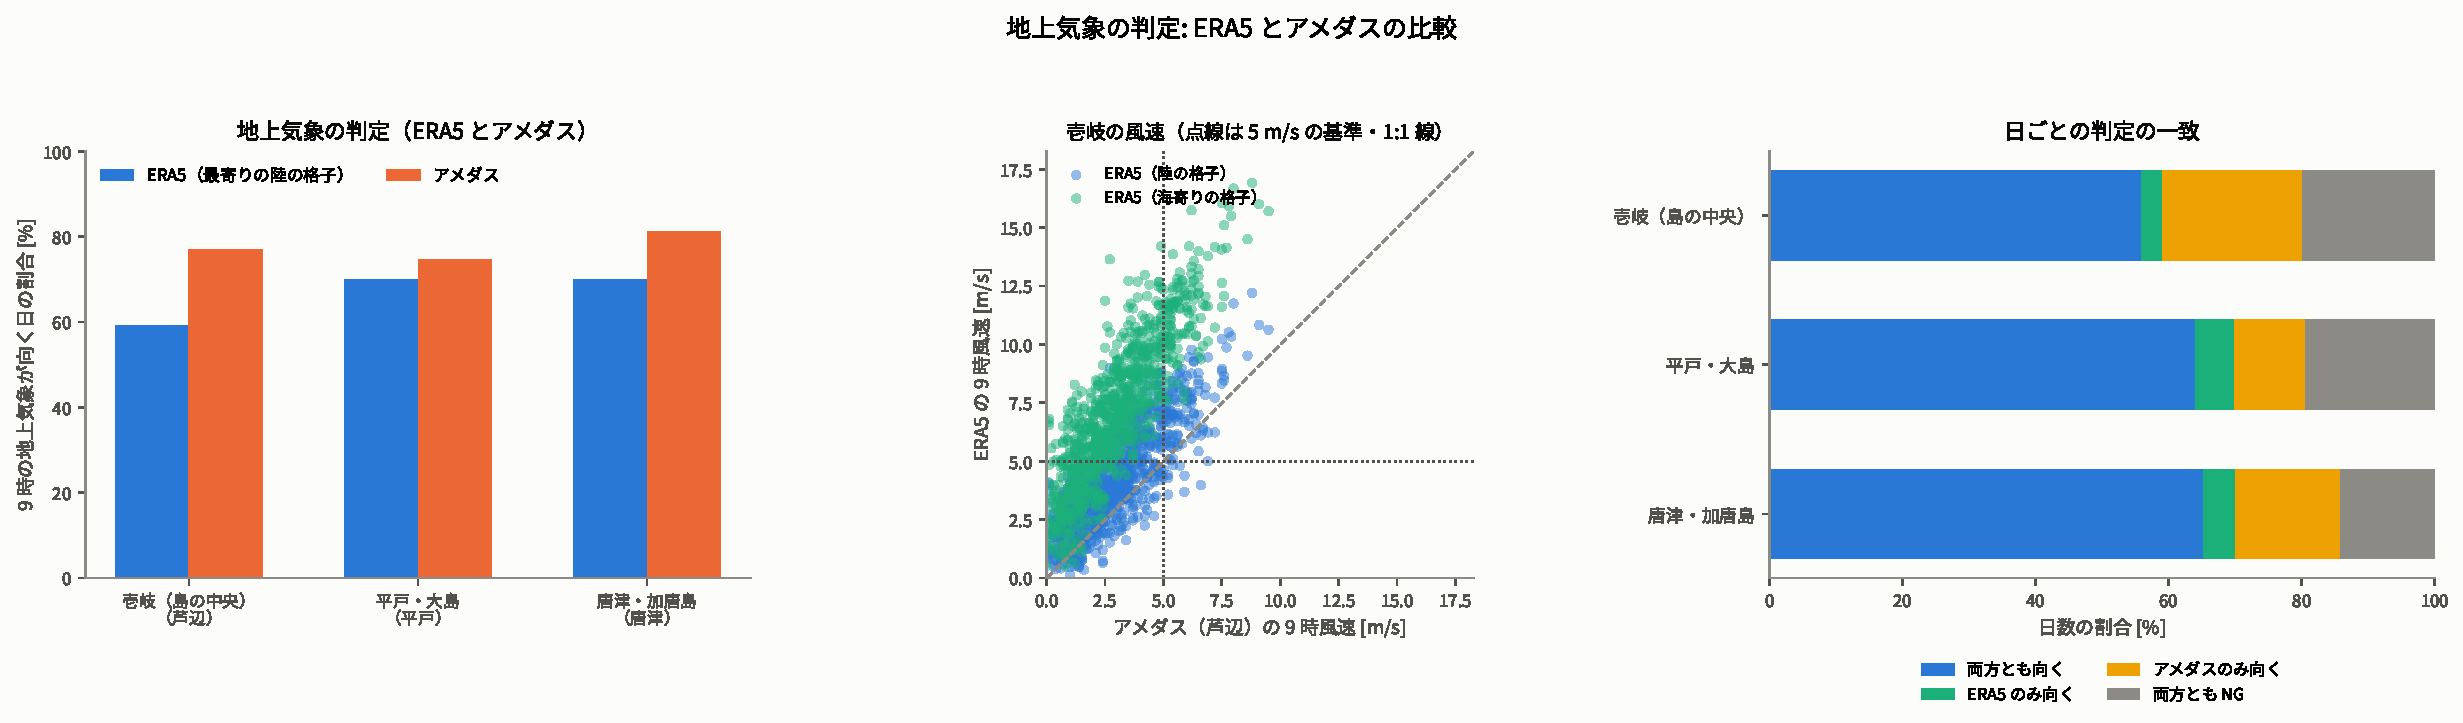
\includegraphics[width=\linewidth]{amedas_compare.pdf}
\caption{9 時の地上気象の比較。(a) 打ち上げに向く日の割合（ERA5 とアメダス）。
(b) 壱岐の 9 時の風速（ERA5 とアメダス芦辺）。(c) 日ごとの判定の一致。}
\label{fig:amedas}
\end{figure}

\subsection{壱岐で実施できる確率と、できない確率}

アメダスで地上気象を判定すると、壱岐から上げて実施できる確率は
\begin{itemize}
  \item 標準の飛行で \textbf{\SI{37}{\percent}}（95\% 区間 34--40）、実施できない確率は \SI{63}{\percent}
  \item 短時間の飛行で \textbf{\SI{49}{\percent}}（46--51）、実施できない確率は \SI{51}{\percent}
\end{itemize}
である。アメダスで計算し直した 4 地点の中では、標準の飛行で最も高い（ただし唐津・加唐島の \SI{36}{\percent} との差は区間の中にある）。
短時間の飛行では唐津・加唐島（\SI{52}{\percent}）とほぼ並ぶ。
つまり\textbf{壱岐は、冬の打ち上げ場所として日本で最も条件の良い場所の 1 つ}である。

実施できない日の内訳を表~\ref{tab:iki} に示す。標準の飛行では、
落下予測が山地（主に山口・福岡・広島の山地）に入って見送る日が \SI{35}{\percent} で最も多く、
地上の風・雨で中止する日が \SI{22}{\percent}、打ち上げ地点の雪は \SI{2}{\percent} である。
短時間の飛行にすると、山地に入る日が \SI{24}{\percent} に減る。

\begin{table}[htbp]
\centering
\small
\caption{壱岐（島の中央、33.78, 129.72）で毎朝 9 時に判断したときの結果の内訳（903 日の割合）。
雪 → 地上気象 → 落下予測の順に判断した。右の列は地上気象を ERA5 で判定した場合。}
\label{tab:iki}
\begin{tabular}{lrrr}
\toprule
& \multicolumn{2}{c}{地上気象: アメダス芦辺} & ERA5 \\
9 時の判断の結果 & 標準 [\%] & 短時間 [\%] & 標準 [\%] \\
\midrule
成功: 瀬戸内海に落ちる & 32.6 & 41.2 & 25.7 \\
成功: 平野に落ちる & 3.2 & 6.2 & 2.5 \\
成功: 海岸から 3 km 以内の海 & 1.2 & 1.2 & 0.9 \\
中止: 打ち上げ地点に雪 & 2.1 & 2.1 & 2.1 \\
中止: 地上の風・雨 & 22.4 & 22.4 & 39.2 \\
見送り: 落下予測が山地 & 35.1 & 24.1 & 27.3 \\
見送り: 落下予測が沖の海 & 2.2 & 1.5 & 1.5 \\
見送り: 落下予測が市街地 & 1.0 & 1.1 & 0.7 \\
見送り: 落下予測地点に雪 & 0.2 & 0.2 & 0.1 \\
\midrule
実施できる（成功の合計） & \textbf{36.9} & \textbf{48.6} & 29.1 \\
\quad 95\% 区間 & 34--40 & 46--51 & 26--32 \\
実施できない & 63.1 & 51.4 & 70.9 \\
\bottomrule
\end{tabular}

\end{table}

\begin{figure}[htbp]
\centering
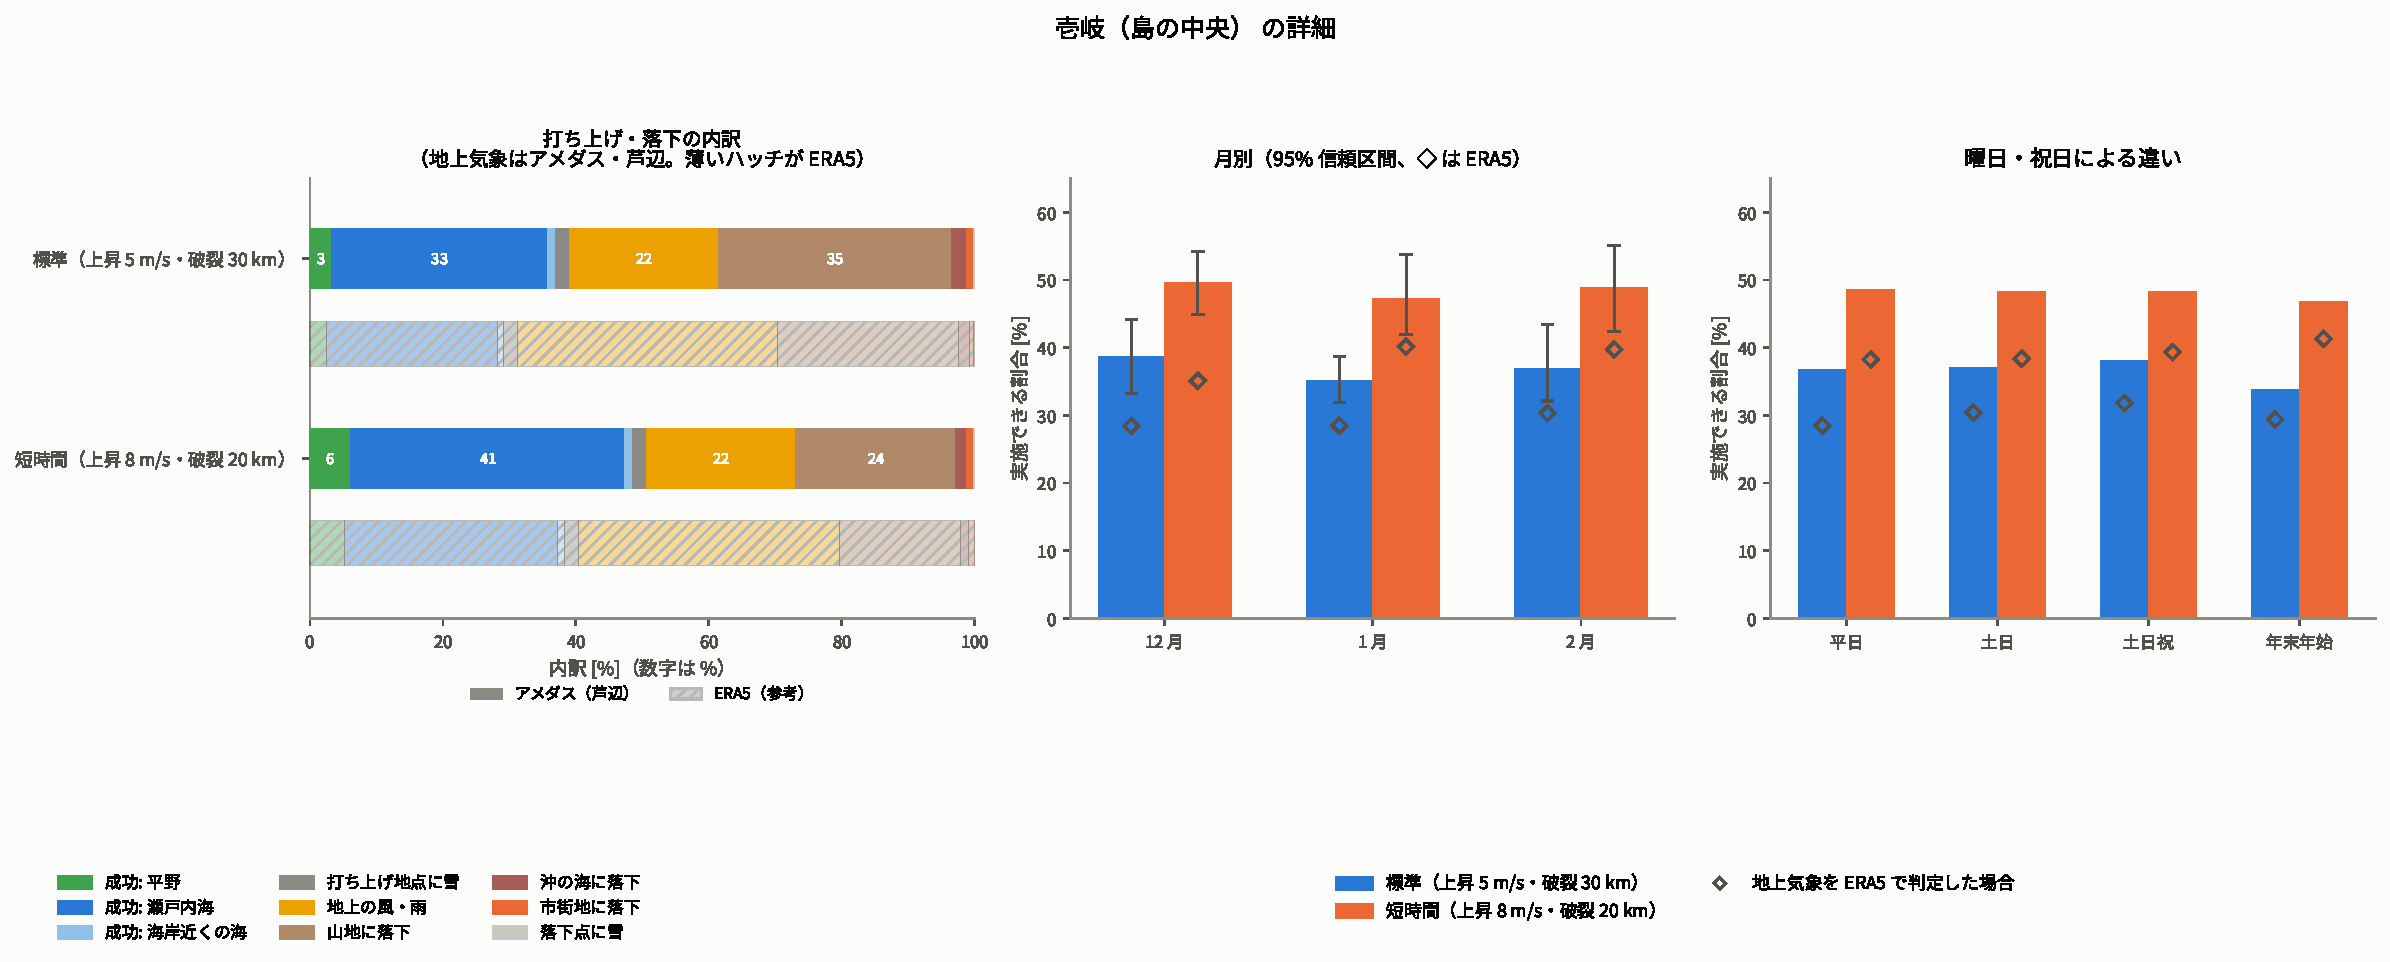
\includegraphics[width=\linewidth]{iki_detail.pdf}
\caption{壱岐の詳細（地上気象はアメダス芦辺）。(a) 9 時の判断の結果の内訳。
(b) 月ごとの実施できる確率（95\% 区間つき）。(c) 平日・土日・土日祝・年末年始の確率。
薄い色は地上気象を ERA5 で判定した場合。}
\label{fig:iki}
\end{figure}

\subsection{壱岐のどこで上げるか}

壱岐島の中で打ち上げに使えそうな広場は 34 か所あり、電線・建物・林から \SI{60}{\metre} 以上
離れられる所は 10 か所ある（図~\ref{fig:spotsiki}、表~\ref{tab:spotsiki}）。
島の中でどこから上げても、実施できる確率は標準の飛行で \SIrange{36}{38}{\percent}、
短時間の飛行で \SIrange{45}{50}{\percent} と、ほとんど変わらない。
壱岐空港（島の南東）の周り \SI{3}{\kilo\metre} は除いた。空港から \SI{9}{\kilo\metre} 以内の所は、
飛行の許可を取るときに空港との調整が要る可能性がある。

\begin{figure}[htbp]
\centering
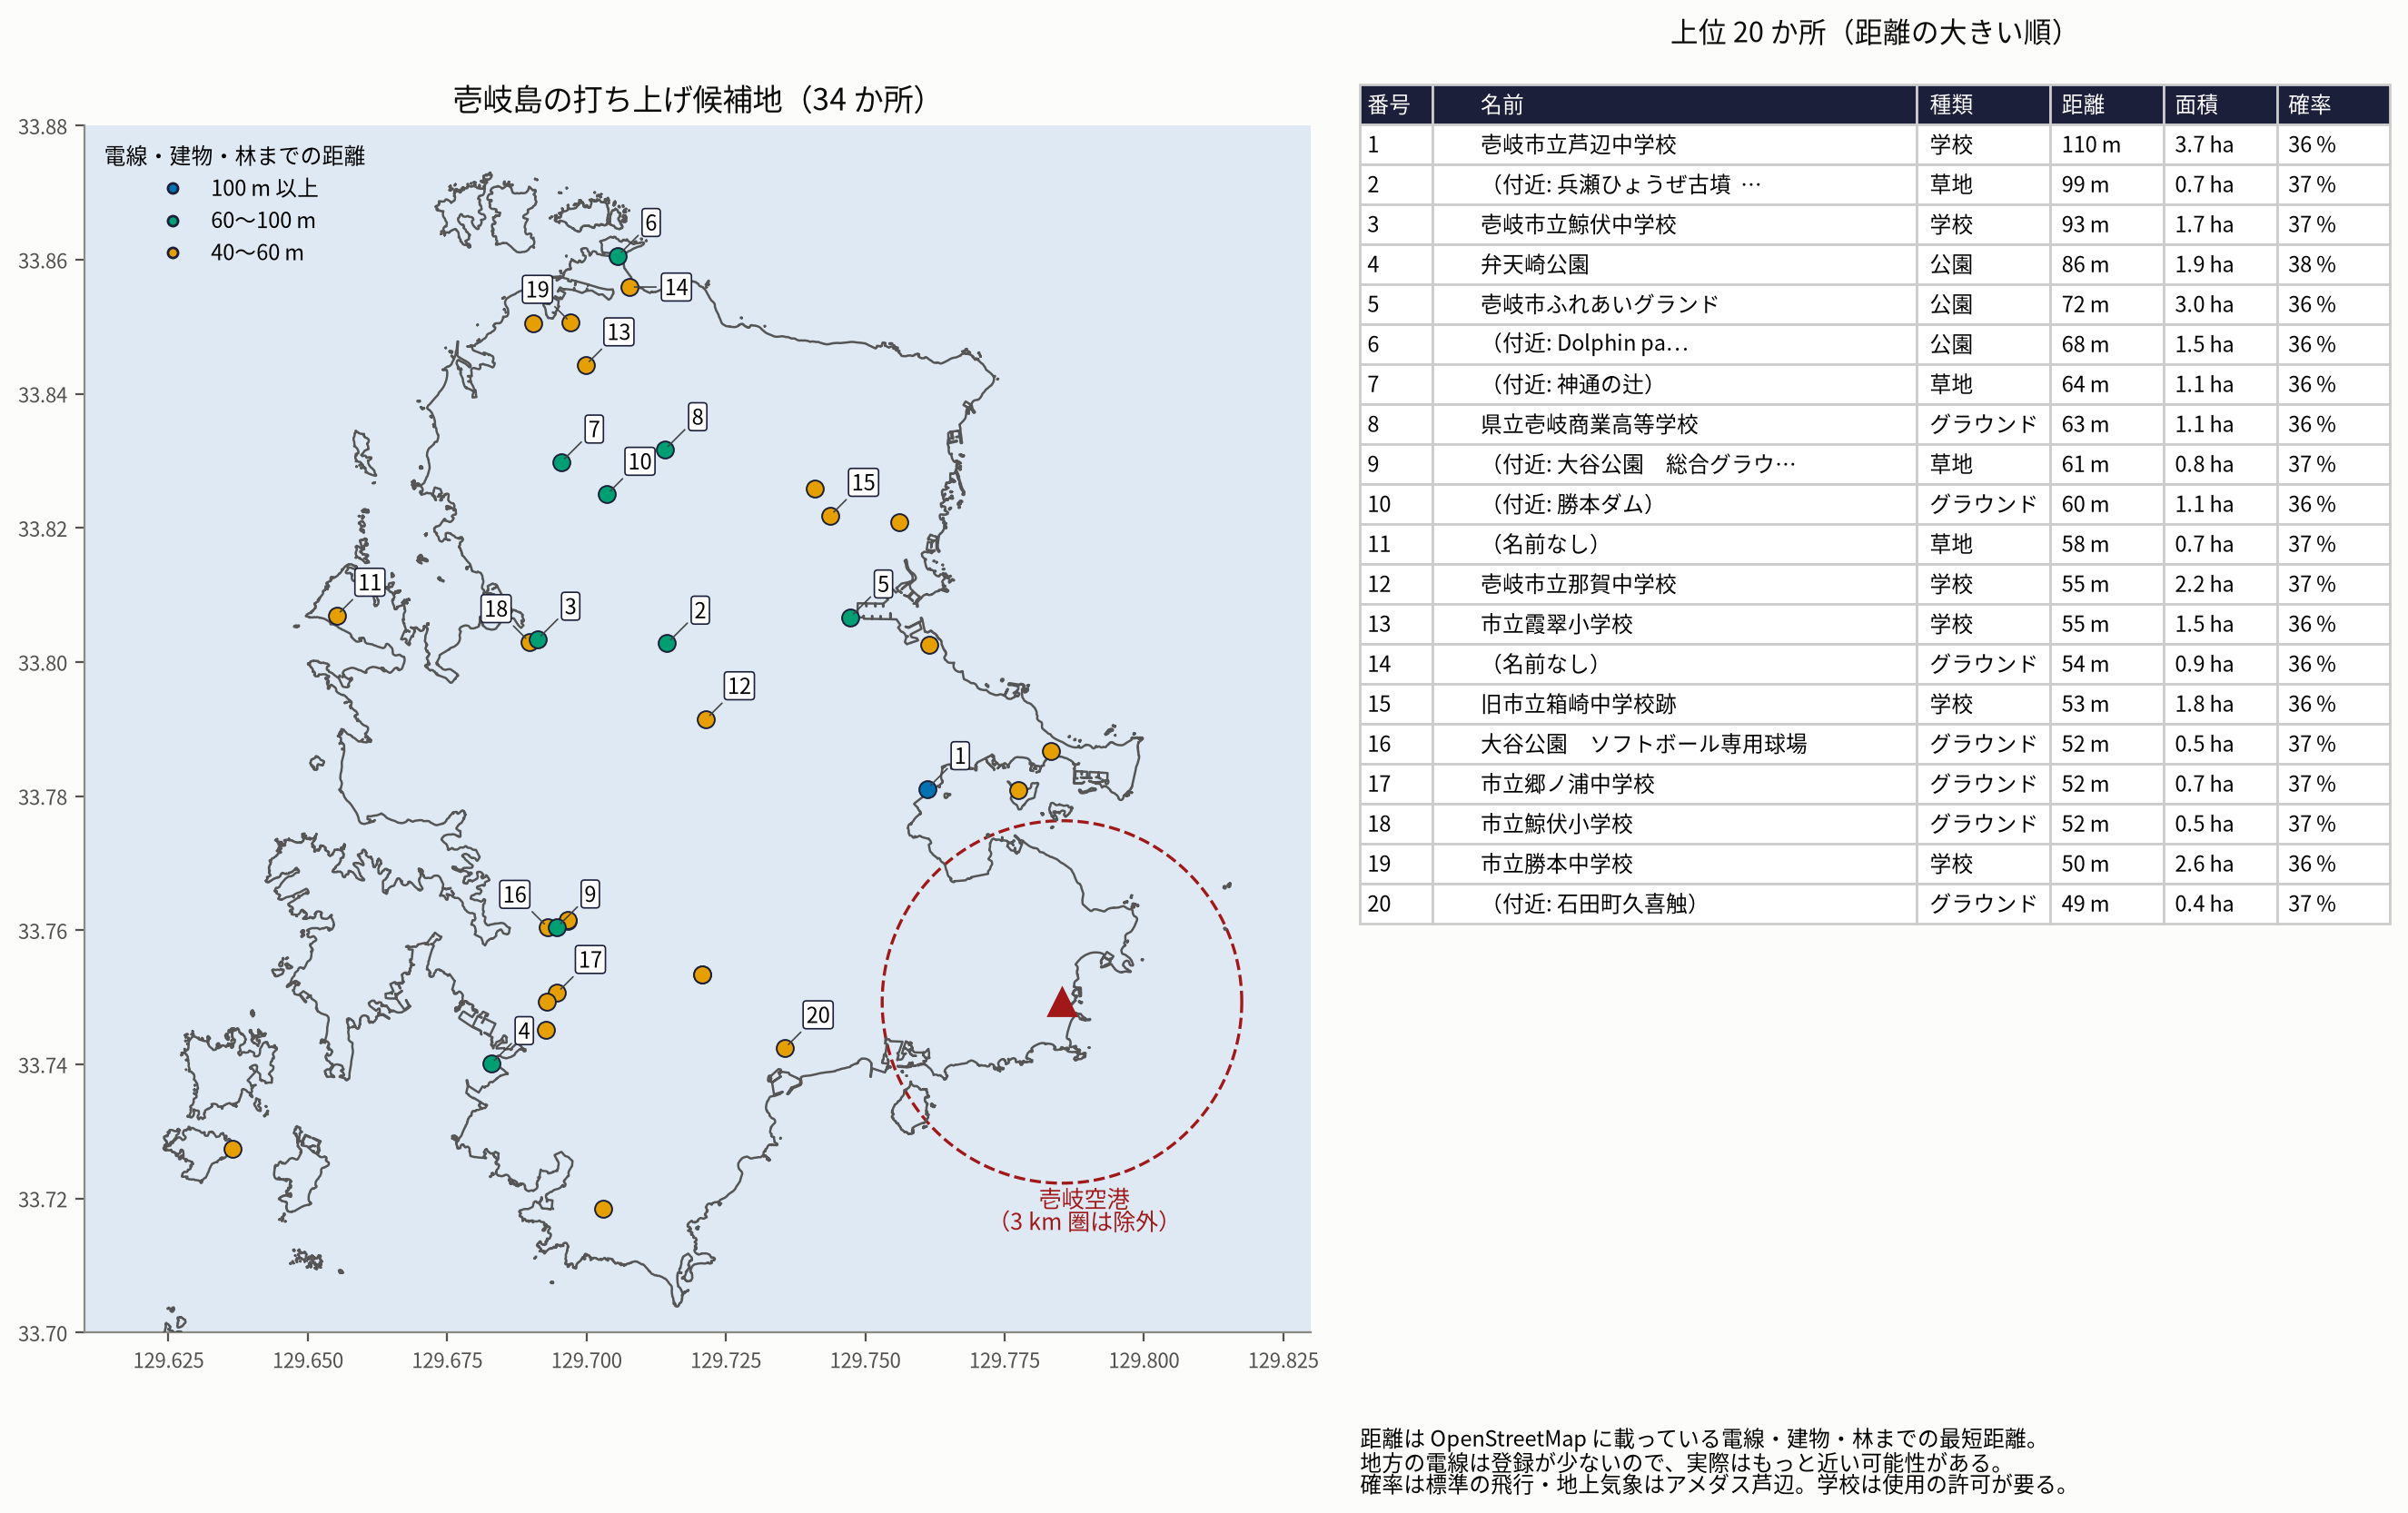
\includegraphics[width=\linewidth]{launch_spots_iki.png}
\caption{壱岐島の打ち上げ候補地。色は電線・建物・林までの距離。番号は右の一覧と対応する。
確率は標準の飛行、地上気象はアメダス芦辺。}
\label{fig:spotsiki}
\end{figure}

\begin{table}[htbp]
\centering
\scriptsize
\caption{壱岐島の打ち上げ候補地（距離の大きい順に 15 か所）。「距離」は電線・建物・林までの距離、
「空港」は壱岐空港の滑走路までの距離、確率は標準 / 短時間の飛行。名前が「付近:」の所は
OpenStreetMap に名前が無く、近くの地名を付けた。}
\label{tab:spotsiki}
\resizebox{\linewidth}{!}{\begin{tabular}{rllcrrrcl}
\toprule
 & 名前 & 種類 & 緯度, 経度 & 距離 [m] & 面積 [ha] & 空港 [km] & 確率 [\%] & \\
\midrule
1 & 壱岐市立芦辺中学校 & 学校 & 33.7811, 129.7611 & 110 & 3.7 & 3.8 & 36 / 49 & 要許可（学校） \\
2 & （付近: 兵瀬ひょうぜ古墳  前方後円墳） & 草地 & 33.8028, 129.7145 & 99 & 0.7 & 8.6 & 37 / 48 &  \\
3 & 壱岐市立鯨伏中学校 & 学校 & 33.8034, 129.6912 & 93 & 1.7 & 10.4 & 37 / 47 & 要許可（学校） \\
4 & 弁天崎公園 & 公園 & 33.7401, 129.6829 & 86 & 1.9 & 9.4 & 38 / 49 &  \\
5 & 壱岐市ふれあいグランド & 公園 & 33.8067, 129.7473 & 72 & 3.0 & 6.9 & 36 / 48 &  \\
6 & （付近: Dolphin park） & 公園 & 33.8606, 129.7056 & 68 & 1.5 & 14.0 & 36 / 45 &  \\
7 & （付近: 神通の辻） & 草地 & 33.8298, 129.6954 & 64 & 1.1 & 11.9 & 36 / 46 &  \\
8 & 県立壱岐商業高等学校 & グラウンド & 33.8316, 129.7140 & 63 & 1.1 & 10.9 & 36 / 46 & 要許可（学校） \\
9 & （付近: 大谷公園　総合グラウンド） & 草地 & 33.7605, 129.6947 & 61 & 0.8 & 8.5 & 37 / 49 &  \\
10 & （付近: 勝本ダム） & グラウンド & 33.8250, 129.7036 & 60 & 1.1 & 11.0 & 36 / 46 &  \\
11 & （名前なし） & 草地 & 33.8069, 129.6552 & 58 & 0.7 & 13.5 & 37 / 47 &  \\
12 & 壱岐市立那賀中学校 & 学校 & 33.7915, 129.7215 & 55 & 2.2 & 7.3 & 37 / 48 & 要許可（学校） \\
13 & 市立霞翠小学校 & 学校 & 33.8443, 129.6999 & 55 & 1.5 & 12.8 & 36 / 46 & 要許可（学校） \\
14 & （名前なし） & グラウンド & 33.8559, 129.7077 & 54 & 0.9 & 13.4 & 36 / 45 &  \\
15 & 旧市立箱崎中学校跡 & 学校 & 33.8218, 129.7437 & 53 & 1.8 & 8.5 & 36 / 47 & 要許可（学校） \\
\bottomrule
\end{tabular}
}
\end{table}

\subsection{壱岐の土日}

\begin{table}[htbp]
\centering
\scriptsize
\caption{壱岐の土日の確率（地上気象はアメダス芦辺）。数え方は \ref{sec:weekend} 節を参照。}
\label{tab:ikiweekend}
\resizebox{\linewidth}{!}{\begin{tabular}{lrrrrrrrrrr}
\toprule
& 全日 & 土日の & 決めた & 週末の & 土曜できた & \multicolumn{2}{c}{1 冬に実施できる [日]} & \multicolumn{3}{c}{毎週末挑戦して [\%]} \\
飛行 & [\%] & 1 日 [\%] & 土曜 [\%] & どちらか [\%] & 日曜も [\%] & 全日 & 土日 & 1 週目 & 2 週以内 & 4 週以内 \\
\midrule
標準 & 37 & 37 & 40 & 58 & 42 & 33.6 & 9.6 & 58 & 82 & 93 \\
短時間 & 49 & 48 & 53 & 71 & 49 & 44.3 & 12.7 & 72 & 92 & 98 \\
\bottomrule
\end{tabular}
}
\end{table}

壱岐（標準の飛行）では、土日の 1 日に実施できる確率が \SI{37}{\percent}、1 回の週末（土日の 2 日）の
どちらかで実施できる確率が \SI{58}{\percent} である（表~\ref{tab:ikiweekend}）。
12--2 月の 1 冬に実施できる日は平均 33.6 日、そのうち土日は 9.6 日ある。
毎週末挑戦すれば、2 週以内に \SI{82}{\percent}、4 週以内に \SI{93}{\percent} の確率で実施できる。
短時間の飛行なら、1 回の週末で \SI{71}{\percent}、2 週以内で \SI{92}{\percent} になる。

島で上げる場合は、機材と人をフェリーで運ぶ日程も週末に合わせる必要がある。
前日の予報で落下予測が山地に入ると分かった週末は、渡航そのものを見送ることになる。

\section{土日に実施できる確率}
\label{sec:weekend}

打ち上げは土日に行うことが多い。そこで、実施できる日が土日に当たる確率を、
2016--2025 年の実際の暦（曜日・祝日）に日ごとの確率を当てはめて数えた。

\subsection{数え方}

\begin{itemize}
  \item \textbf{土日の 1 日}: 土曜または日曜の 1 日を選んだとき、その日に実施できる確率。
  \item \textbf{決めた土曜}: 何か月も前に「この土曜」と決めた場合の確率。
  \item \textbf{土日のどちらか}: 1 回の週末（土・日の 2 日）のうち、どちらかの日に実施できる確率。
    両日とも挑戦できる前提。
  \item \textbf{土曜に実施できたとき日曜も}: 天気は続くので、土曜と日曜は独立ではない。
    この値が「土日の 1 日」より高ければ、良い日はまとまって来る。
  \item \textbf{1 冬に実施できる土日}: 12--2 月の約 26 日の土日のうち、実施できる日数の期待値。
  \item \textbf{毎週末挑戦して $N$ 週以内}: ある週末から毎週末（土日の両日）挑戦したとき、
    $N$ 回目の週末までに実施できる確率。12--2 月のどの週末から始めても同じ重みで数え、
    2 月末で打ち切った。
\end{itemize}

飛行条件のばらつきによる成否は日ごとに独立な乱数で決めた。天気そのものは実際の日の
並びをそのまま使っているので、悪天候が何日も続く効果は入っている。

\begin{table}[htbp]
\centering
\scriptsize
\caption{土日の確率。上が標準の飛行、下が短時間の飛行。}
\label{tab:weekend}
\resizebox{\linewidth}{!}{\begin{tabular}{llrrrrrrr}
\toprule
飛行 & 候補地 & 土日の & 決めた土曜 & 土日の & 土曜に実施 & 1 冬に実施 & \multicolumn{2}{c}{毎週末挑戦して} \\
& & 1 日 [\%] & 1 日 [\%] & どちらか [\%] & できたとき & できる土日 & 2 週以内 & 4 週以内 \\
& & & & & 日曜も [\%] & [日] & [\%] & [\%] \\
\midrule
標準 & 壱岐（島の中央） & 30 & 34 & 49 & 38 & 7.8 & 71 & 88 \\
標準 & 平戸・大島 & 33 & 36 & 53 & 37 & 8.5 & 73 & 90 \\
標準 & 唐津・加唐島 & 35 & 38 & 54 & 40 & 8.8 & 74 & 91 \\
標準 & 下関・蓋井島 & 33 & 38 & 54 & 37 & 8.6 & 77 & 91 \\
標準 & 山口・徳地 & 35 & 36 & 55 & 42 & 9.0 & 78 & 92 \\
標準 & 糸島・志摩 & 28 & 28 & 45 & 39 & 7.0 & 63 & 82 \\
標準 & 福津 & 25 & 25 & 40 & 37 & 6.1 & 58 & 78 \\
標準 & 廿日市 & 32 & 34 & 51 & 41 & 8.3 & 72 & 88 \\
\midrule
短時間 & 壱岐（島の中央） & 38 & 44 & 60 & 40 & 10.0 & 86 & 97 \\
短時間 & 平戸・大島 & 34 & 38 & 54 & 36 & 8.7 & 75 & 90 \\
短時間 & 唐津・加唐島 & 46 & 50 & 69 & 45 & 12.2 & 90 & 97 \\
短時間 & 下関・蓋井島 & 35 & 37 & 56 & 42 & 9.5 & 82 & 93 \\
短時間 & 山口・徳地 & 38 & 41 & 59 & 46 & 10.2 & 85 & 96 \\
短時間 & 糸島・志摩 & 48 & 51 & 70 & 52 & 12.3 & 89 & 98 \\
短時間 & 福津 & 45 & 46 & 65 & 54 & 11.5 & 85 & 96 \\
短時間 & 廿日市 & 47 & 52 & 67 & 52 & 12.3 & 90 & 98 \\
\bottomrule
\end{tabular}
}
\end{table}

\subsection{結果}

曜日によって天気が変わるわけではないので、「土日の 1 日」は全日の確率とほぼ同じになる。
以下は全地点を同じ方法（地上気象は ERA5）で比べた値である。壱岐のアメダスによる値は
表~\ref{tab:ikiweekend} にある。

壱岐（標準の飛行、ERA5）では、土日の 1 日で \SI{30}{\percent}、1 回の週末のどちらかで
\SI{49}{\percent} である。土曜に実施できた週末に日曜も実施できる確率は \SI{38}{\percent} で、
1 日の確率（\SI{30}{\percent}）より高い。良い日は 2 日続きやすい。

1 冬の 12--2 月に、壱岐で実施できる土日は平均 7.8 日ある。毎週末挑戦すると、
2 週以内に \SI{71}{\percent}、4 週以内に \SI{88}{\percent} の確率で実施できる。
短時間の飛行にすると 2 週以内が \SI{86}{\percent}、4 週以内が \SI{97}{\percent} に上がる。

\textbf{日程を 1 日に固定すると約 3 割、週末の 2 日にしても約 5 割にとどまる}。
予備日として同じ週末の 2 日と、その後の 2--3 週末を確保しておくのが現実的である。

\begin{figure}[htbp]
\centering
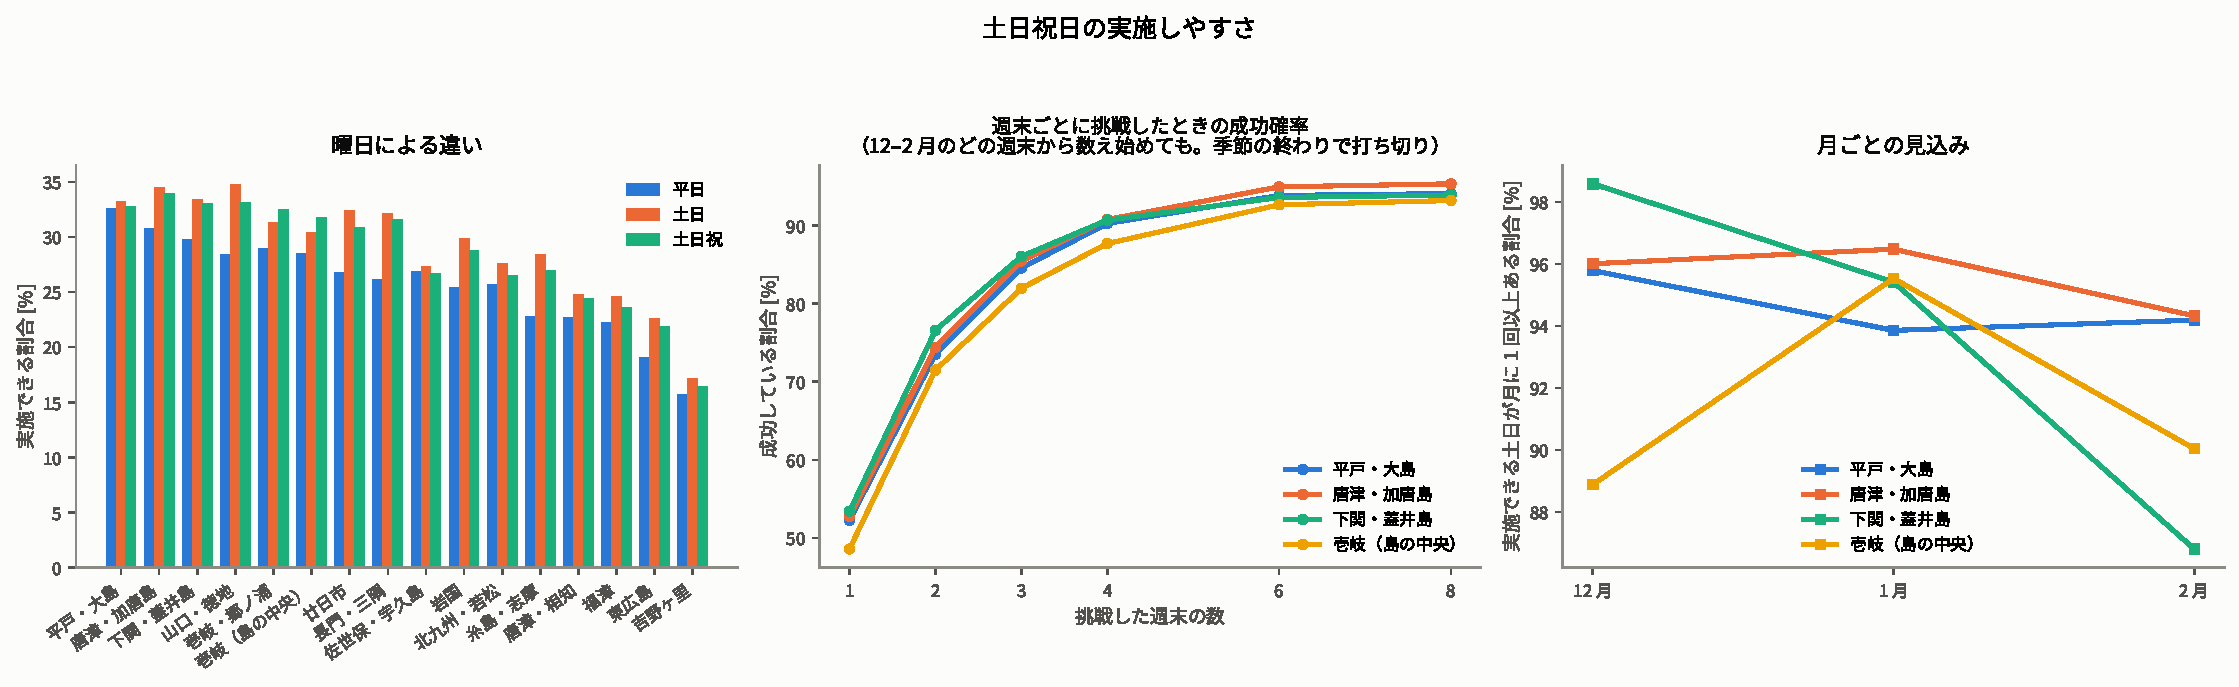
\includegraphics[width=\linewidth]{weekend.pdf}
\caption{土日の確率。(a) 平日・土日・土日祝の 1 日あたりの確率。(b) 毎週末挑戦したとき、
$N$ 回目の週末までに実施できる確率。(c) 各月に実施できる土日が 1 日以上ある確率。}
\label{fig:weekend}
\end{figure}

\begin{figure}[htbp]
\centering
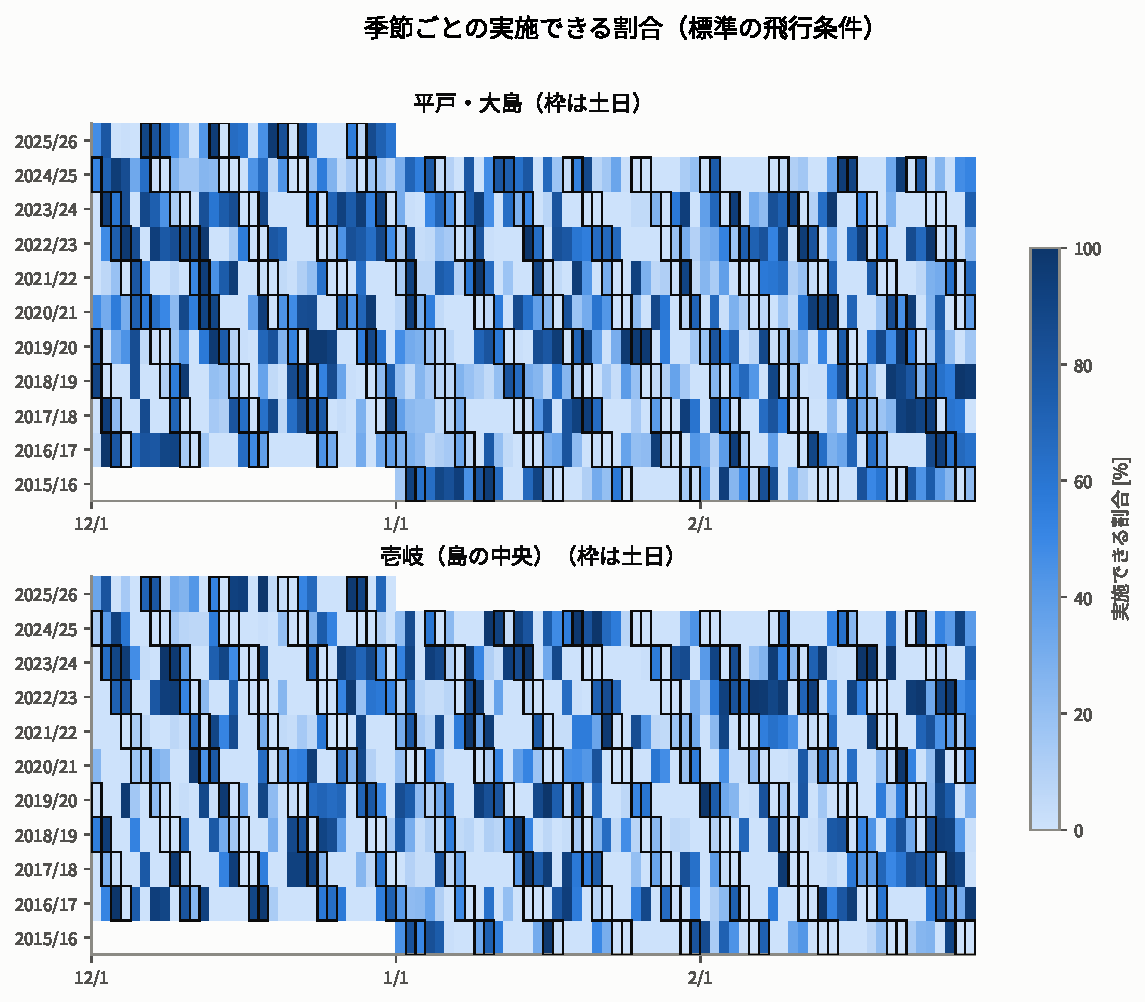
\includegraphics[width=\linewidth]{calendar.pdf}
\caption{日ごとの実施できる確率（標準の飛行）。行が冬（12 月〜翌 2 月）、列が日付。
印は土日。良い日と悪い日がそれぞれ数日ずつかたまって現れる。}
\label{fig:calendar}
\end{figure}

\subsection{月と年による違い}

\begin{table}[htbp]
\centering
\scriptsize
\caption{月ごとの実施できる確率と、年末年始（12 月 29 日〜1 月 3 日）の確率。}
\label{tab:months}
\begin{tabular}{lrrrrrrrr}
\toprule
& \multicolumn{3}{c}{標準 [\%]} & \multicolumn{3}{c}{短時間 [\%]} & \multicolumn{2}{c}{年末年始 [\%]} \\
候補地 & 12 月 & 1 月 & 2 月 & 12 月 & 1 月 & 2 月 & 標準 & 短時間 \\
\midrule
壱岐（島の中央） & 28 & 28 & 30 & 35 & 40 & 40 & 29 & 41 \\
平戸・大島 & 36 & 29 & 33 & 37 & 32 & 33 & 35 & 44 \\
唐津・加唐島 & 34 & 29 & 33 & 46 & 45 & 44 & 32 & 58 \\
下関・蓋井島 & 34 & 29 & 30 & 35 & 37 & 35 & 30 & 44 \\
山口・徳地 & 34 & 28 & 28 & 36 & 34 & 36 & 34 & 38 \\
糸島・志摩 & 27 & 23 & 23 & 50 & 46 & 49 & 21 & 55 \\
福津 & 26 & 22 & 20 & 44 & 43 & 44 & 25 & 43 \\
廿日市 & 32 & 26 & 28 & 46 & 42 & 41 & 29 & 47 \\
\bottomrule
\end{tabular}

\end{table}

月による違いは小さく、12 月・1 月・2 月のどれでも大きくは変わらない（表~\ref{tab:months}）。
一方、年による違いは月による違いより大きい（図~\ref{fig:byyear}）。壱岐（標準の飛行）でも、
実施できる確率は \SI{21}{\percent} の年（2021 年）から \SI{39}{\percent} の年（2023 年）まで開く。
1 回の冬の経験で場所の良し悪しを判断しないほうがよい。

\begin{figure}[htbp]
\centering
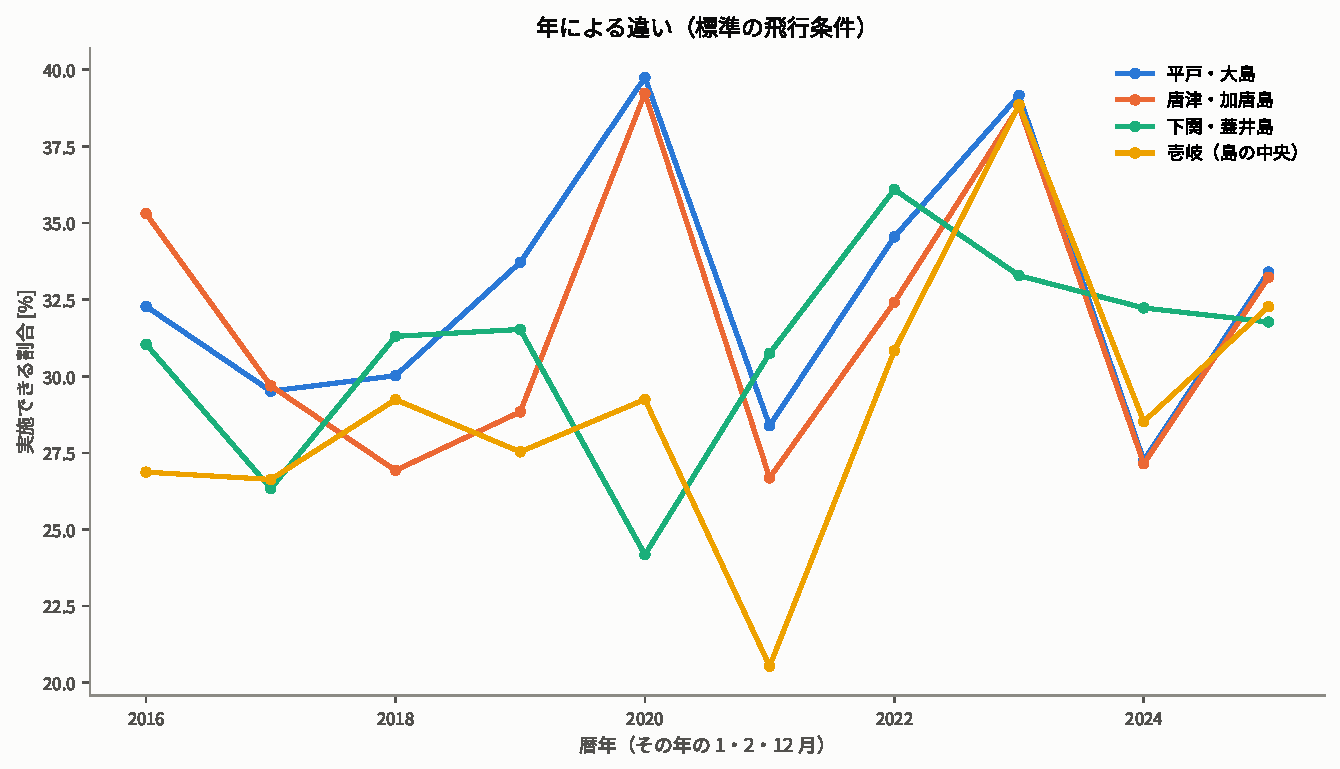
\includegraphics[width=\linewidth]{by_year.pdf}
\caption{年ごとの実施できる確率（その年の 1・2・12 月。冬のシーズンではなく暦年で分けた）。}
\label{fig:byyear}
\end{figure}

\section{判定の基準を変えたとき}
\label{sec:sensitivity}

判定の基準は、どれもある程度は任意に決めた値である。値を 1 つずつ変えて、
標準の飛行で実施できる確率がどれだけ動くかを調べた（図~\ref{fig:sens}）。

\begin{description}
  \item[地上の風の上限] 最も効く。壱岐では上限を \SI{5}{\metre\per\second} から
    \SI{3}{\metre\per\second} に下げると \SI{29}{\percent} が \SI{15}{\percent} に半減し、
    \SI{7}{\metre\per\second} に上げると \SI{37}{\percent} になる。放球の技術と機材で
    許せる風速を決めることが、場所を選ぶことと同じくらい確率を左右する。
  \item[海岸から何 km までの海を認めるか] 0 km（瀬戸内海だけ）から \SI{10}{\kilo\metre} まで
    変えても、壱岐では \SIrange{28}{30}{\percent} とほとんど動かない。
    冬は落下点の多くが瀬戸内海か山地で、外海の海岸近くに落ちる日は少ないからである。
    平戸・大島と唐津・加唐島は \SIrange{30}{36}{\percent} と少し動く。
  \item[降水の上限] 9--12 時の降水を \SI{0.1}{\milli\metre} 未満にすると
    \SIrange{2}{4}{\percent} 下がり、\SI{2}{\milli\metre} 未満に緩めると同じくらい上がる。
  \item[瀬戸内海への着水] 認めない場合は、成功が平野と海岸近くの海だけになる。
    壱岐では実施できる確率が \SI{29}{\percent} から \SI{3}{\percent} 程度に、
    他の上位地点も \SIrange{3}{12}{\percent} に下がる（図~\ref{fig:breakdown} の成功の内訳）。
    瀬戸内海を使えないと、冬の西風で東へ \SI{250}{\kilo\metre} 流される先に、
    雪のない平野がまとまって広がる場所がほとんどない。
\end{description}

\begin{figure}[htbp]
\centering
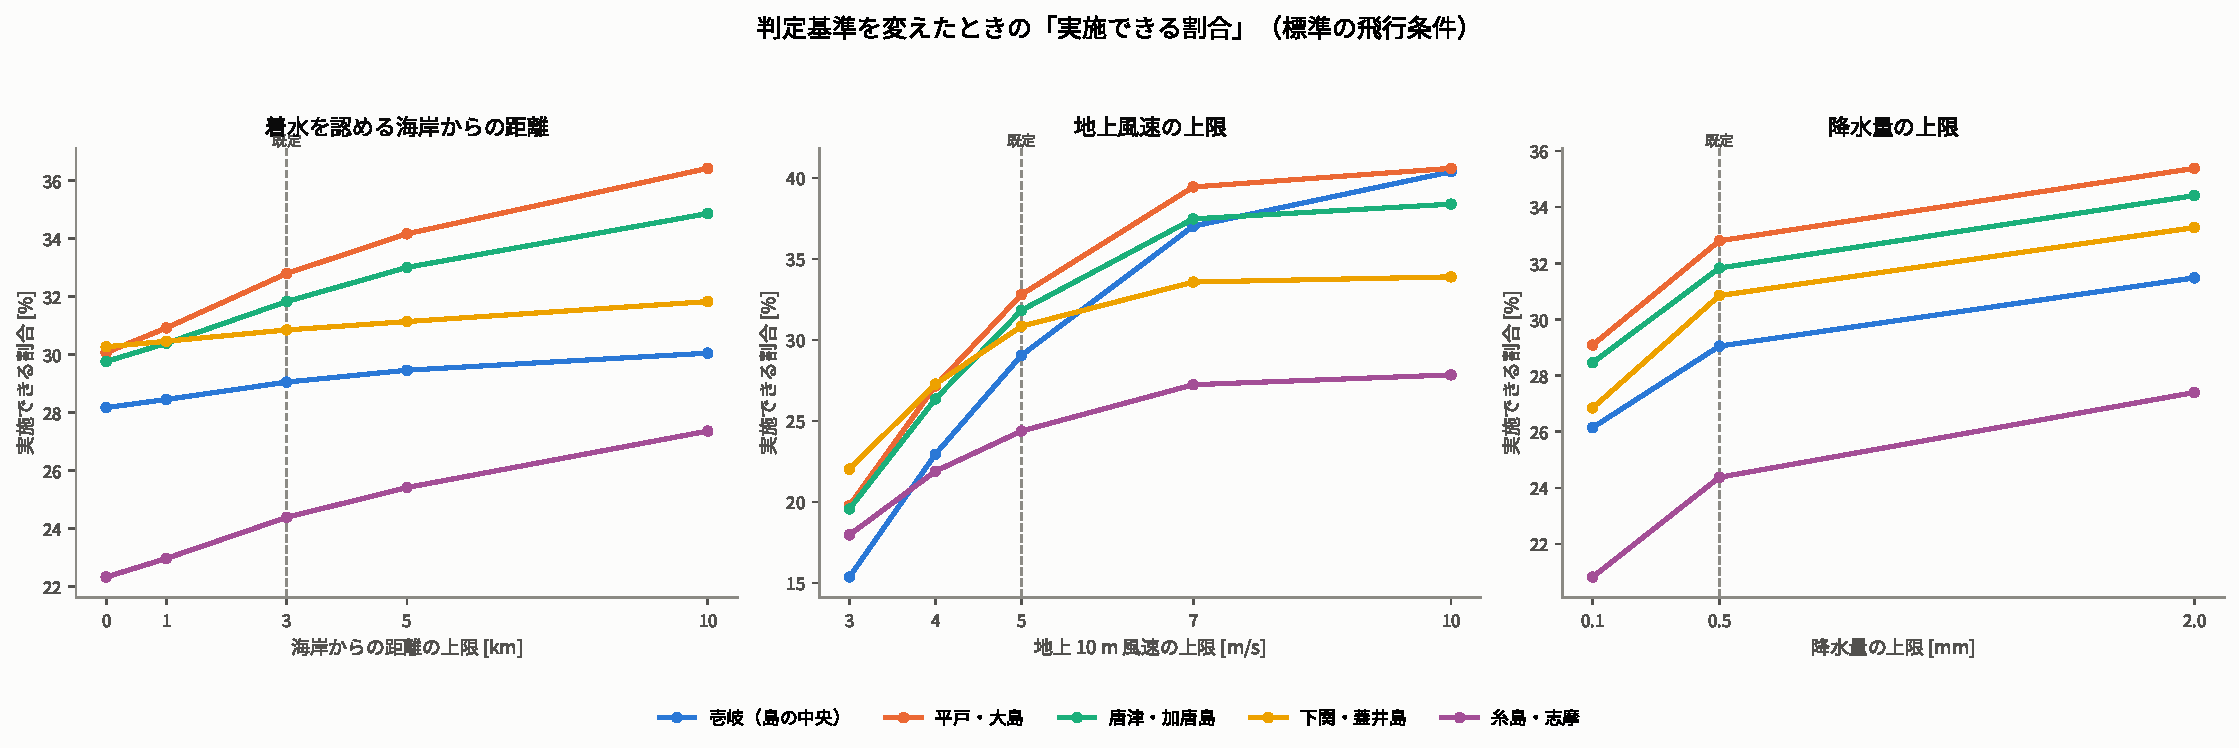
\includegraphics[width=\linewidth]{sensitivity.pdf}
\caption{判定の基準を変えたときの実施できる確率（標準の飛行）。
破線が本文で使った値（海岸から \SI{3}{\kilo\metre}、風 \SI{5}{\metre\per\second}、
降水 \SI{0.5}{\milli\metre}）。}
\label{fig:sens}
\end{figure}

\section{この結果で言えないこと}
\label{sec:limits}

\begin{enumerate}
  \item \textbf{確率は過去 10 年の割合である}。将来の冬が同じ割合になる保証はない。
    年による違い（図~\ref{fig:byyear}）が \SI{\pm 10}{\percent} ほどあるので、
    1 冬で経験する割合はこの範囲で上下する。
  \item \textbf{予報が当たる前提で数えている}。実際の判断は前日から当日朝の予報で行う。
    予報の落下点がずれて、目標に入るはずが山に落ちる日や、その逆の日が出る。
    予報の誤差はこの計算に入っていない。目標の縁に近い日ほど、予報と実際で成否が入れ替わりやすい。
  \item \textbf{地上気象は \ang{0.25}（約 \SI{25}{\kilo\metre}）格子の値である}。
    島や海岸では、格子に海が混ざるかどうかで地上の風が大きく変わる（\ref{sec:amedas} 節）。
    本文では最寄りの陸の格子を使ったが、実際の打ち上げ場所の風は地形や建物で
    さらに変わる。現地の風の記録で確かめる必要がある。
  \item \textbf{9 時の 1 回だけを見ている}。朝の風が強くても昼に弱まる日は、実際には
    時刻をずらして上げられる。そのぶん実施できる確率は本文の値より高い可能性がある。
    逆に、日没までに回収を終える時間の制約は入れていない。
  \item \textbf{上空の風は JRA-3Q の \ang{0.375} 格子・6 時間ごとの解析値である}。
    飛行中の風の時間変化（約 2 時間）は入れていない。
  \item \textbf{瀬戸内海への着水の扱い}。瀬戸内海に落ちた機体を回収できるか、
    船舶の多い海域に落としてよいかは、この計算の外の問題である。
    上位の候補地では成功の 7--9 割が瀬戸内海への着水なので、これを認めるかどうかで結論が変わる。
  \item \textbf{平野の定義は地形だけで決めている}。水田・畑・森林・河川・道路の区別はしていない。
    冬の水田は回収しやすいが、ため池や河川に落ちることもある。
  \item \textbf{航空法などの手続き}は考えていない。空港の周辺や航空路の下では
    飛行の許可が必要で、候補地によっては条件が付く。
\end{enumerate}

\section*{データの出典}
\begin{itemize}
  \item 上空の風: JRA-3Q（気象庁）。NSF NCAR GDEX（d640000）から取得。
  \item 積雪・地上気象: ERA5（Copernicus Climate Change Service）。NSF NCAR GDEX（d633000）から取得。
    Copernicus Climate Change Service の情報を加工したものを含む。
  \item 地上の観測: 気象庁 アメダス（過去の気象データ）。
  \item 地形: NOAA NCEI DEM mosaic。
  \item 市街地: 国土交通省 国土数値情報（人口集中地区データ、2020 年）。
  \item 広場: \textcopyright{} OpenStreetMap contributors（ODbL）。
\end{itemize}
JRA-3Q から作った図と数値は、元データの条件（CC BY-NC-SA 4.0、非商用）に従う。


\end{document}
